%%----------------------------------------------------------------------------
%%
%%                                   Sean Mauch
%%                       California Institute of Technology
%%                        @ 1995-2002 No Rights Reserved
%%
%%----------------------------------------------------------------------------

\flushbottom

%% CONTINUE
%% Add results to this chapter.

%%============================================================================
%%============================================================================
\chapter{Series and Convergence}
\label{chapter_sc}
\index{series}
\index{series!convergence of}




You are not thinking. You are merely being logical.

\begin{flushright}
  - Neils Bohr
\end{flushright}





%%============================================================================
\section{Series of Constants}


%%----------------------------------------------------------------------------
\subsection{Definitions}


\paragraph{Convergence of Sequences.}
\index{sequences!convergence of}
\index{convergence!sequences}
The infinite sequence $\{a_n\}_{n=0}^\infty \equiv a_0, a_1, a_2, \ldots$ 
is said to converge if
\[ 
\lim_{n \to \infty} a_n = a
\]
for some constant $a$.
If the limit does not exist, then the sequence diverges.
Recall the definition of the limit in the above formula:  For any
$\epsilon > 0$ there exists an $N \in \mathbb{Z}$ such that
$|a - a_n| < \epsilon$ for all $n > N$.



\begin{Example}
  The sequence $\{ \sin(n) \}$ is divergent.  The sequence 
  is bounded above and below, but boundedness does not imply convergence.
\end{Example}




\paragraph{Cauchy Convergence Criterion.}
\index{convergence!Cauchy}
\index{Cauchy convergence}
Note that there is something a little fishy about the above definition.
We should be able to say if a sequence converges without first finding the 
constant to which it converges.  We fix this problem with the
\textit{Cauchy convergence criterion}.
A sequence $\{a_n\}$ converges if and only if for any $\epsilon > 0$ there 
exists an $N$ such that $|a_n - a_m| < \epsilon$ for all $n,m > N$.  The Cauchy 
convergence criterion is equivalent to the definition we had before.
For some problems it is handier to use.  Now we don't need to know 
the limit of a sequence to show that it converges.



\paragraph{Convergence of Series.}
\index{series!convergence of}
\index{convergence!series}
The series $\sum_{n = 1}^\infty a_n$ converges if the sequence of \textit{partial sums}, 
$S_N = \sum_{n=0}^{N-1} a_n$,
converges.  That is,
\[ 
\lim_{N \to \infty} S_N = 
\lim_{N \to \infty} \sum_{n=0}^{N-1} a_n = \mathrm{constant}.
\]
If the limit does not exist, then the series diverges.
A necessary condition for the convergence of a series is that
\[ 
\lim_{n \to \infty} a_n = 0.
\]
(See Exercise~\ref{exercise lim an = 0 necessary series convergence}.)
Otherwise the sequence of partial sums would not converge.




\begin{Example}
  The series $\sum_{n = 0}^\infty (-1)^n = 1 - 1 + 1 - 1 + \cdots$ is divergent because 
  the sequence of partial sums, $\{ S_N \} = 1, 0, 1, 0, 1, 0, \ldots$ 
  is divergent.
\end{Example}




\paragraph{Tail of a Series.}
\index{series!tail of}
An infinite series, $\sum_{n=0}^\infty a_n$, converges or diverges with its tail.
That is, for fixed $N$,  $\sum_{n=0}^\infty a_n$ converges if and only if 
$\sum_{n=N}^\infty a_n$ converges.  This is because the sum of the first 
$N$ terms of a series is just a number.  Adding or subtracting a number to 
a series does not change its convergence.





\paragraph{Absolute Convergence.}
\index{absolute convergence}
\index{convergence!absolute}
The series $\sum_{n = 0}^\infty a_n$ converges absolutely if $\sum_{n = 0}^\infty |a_n|$
converges.  Absolute convergence implies convergence.  If a series is
convergent, but not absolutely convergent, then it is said to be 
\textit{conditionally convergent}.

The terms of an absolutely convergent series can be rearranged in any order
and the series will still converge to the same sum.  This is not true of
conditionally convergent series.  Rearranging the terms of a conditionally
convergent series may change the sum.  In fact, the terms of a conditionally
convergent series may be rearranged to obtain any desired sum.



\begin{Example}
  The alternating harmonic series,
  \[ 
  1 - \frac{1}{2} + \frac{1}{3} - \frac{1}{4} + \cdots, 
  \]
  converges, (Exercise~\ref{exercise alternating harmonic series}).
  Since
  \[ 
  1 + \frac{1}{2} + \frac{1}{3} + \frac{1}{4} + \cdots 
  \]
  diverges, (Exercise~\ref{exercise divergent harmonic series}),
  the alternating harmonic series is not absolutely convergent.
  Thus the terms can be rearranged to obtain any sum,
  (Exercise~\ref{exercise rearrange alternating harmonic series}).
\end{Example}






\paragraph{Finite Series and Residuals.}
\index{residuals!of series}
\index{series!residuals}
Consider the series $f(z) = \sum_{n = 0}^\infty a_n(z)$.  We will denote the sum 
of the first $N$ terms in the series as
\[ 
S_N(z) = \sum_{n=0}^{N-1} a_n(z).
\]
We will denote the \textit{residual} after $N$ terms as
\[ 
R_N(z) \equiv f(z) - S_N(z) = \sum_{n=N}^\infty a_n(z).
\]









%%-----------------------------------------------------------------------------
\subsection{Special Series}




\paragraph{Geometric Series.}
\index{geometric series}
\index{series!geometric}
One of the most important series in mathematics is the 
\textit{geometric series},
\footnote{
  The series is so named because the terms grow or decay geometrically.  
  Each term in the series is a constant times the previous term.
  }
\[ 
\sum_{n = 0}^\infty z^n = 1 + z + z^2 + z^3 + \cdots.
\]
The series clearly diverges for $|z| \geq 1$ since the terms do not vanish
as $n \to \infty$.  Consider the partial sum,
$S_N(z) \equiv \sum_{n=0}^{N-1} z^n$, for $|z| < 1$.
\begin{align*}
  (1 - z) S_N(z) &= (1-z) \sum_{n=0}^{N-1} z^n 
  \\
  &= \sum_{n=0}^{N-1} z^n - \sum_{n=1}^{N} z^n 
  \\
  &= \left( 1 + z + \cdots + z^{N-1} \right) - \left( z + z^2 + \cdots + z^N \right) 
  \\
  &= 1 - z^N
\end{align*}
\[ 
\sum_{n=0}^{N-1} z^n = \frac{1 - z^N}{1-z} \to \frac{1}{1 - z} \quad \mathrm{as}\ N \to \infty.
\]
The limit of the partial sums is $\frac{1}{1-z}$.
\[ 
\sum_{n = 0}^\infty z^n = \frac{1}{1-z} \quad \mathrm{for}\ |z| < 1
\]





\paragraph{Harmonic Series.}
\index{harmonic series}
\index{Riemann zeta function}
Another important series is the \textit{harmonic series}, 
\[ 
\sum_{n=1}^\infty \frac{1}{n^\alpha} = 1 + \frac{1}{2^\alpha} + \frac{1}{3^\alpha} + \cdots.
\]
The series is absolutely convergent for $\Re(\alpha) > 1$ and absolutely divergent
for $\Re(\alpha) \leq 1$, (see the Exercise~\ref{exercise harmonic series}).  The 
\textit{Riemann zeta function} $\zeta(\alpha)$ is 
defined as the sum of the harmonic series.
\[ 
\zeta(\alpha) = \sum_{n=1}^\infty \frac{1}{n^\alpha} 
\]
The \textit{alternating harmonic series} is
\[ 
\sum_{n=1}^\infty \frac{(-1)^{n+1}}{n^\alpha} = 1 - \frac{1}{2^\alpha} + \frac{1}{3^\alpha} - \frac{1}{4^\alpha} +  \cdots.
\]
Again, the series is absolutely convergent for $\Re(\alpha) > 1$
and absolutely divergent for $\Re(\alpha) \leq 1$.  
%% CONTINUE: consider conditional convergence.






%%-----------------------------------------------------------------------------
\subsection{Convergence Tests}



\subsubsection{The Comparison Test.}
\index{comparison test}
\index{series!comparison test}
\index{convergence!comparison test}

\begin{Result}
  The series of positive terms $\sum a_n$ converges if there 
  exists a convergent series $\sum b_n$ such that 
  $a_n \leq b_n$ for all $n$.
  Similarly, $\sum a_n$ diverges if there exists a divergent series
  $\sum b_n$ such that $a_n \geq b_n$ for all $n$.
\end{Result}




\begin{Example}
  Consider the series
  \[
  \sum_{n = 1}^\infty \frac{1}{2^{n^2}}.
  \]
  We can rewrite this as 
  \[
  \sum_{\substack{ n=1 \\ n\ \mathrm{a perfect square}}}^\infty \frac{1}{2^n}.
  \]
  Then by comparing this series to the geometric series,
  \[
  \sum_{n = 1}^\infty \frac{1}{2^n} = 1,
  \]
  we see that it is convergent.
\end{Example}












\subsubsection{Integral Test.}
\index{convergence!integral test}
\index{series!integral test}

\begin{Result}
  If the coefficients $a_n$ of a series $\sum_{n=0}^\infty a_n$ are monotonically 
  decreasing and can be extended to a monotonically decreasing function 
  of the continuous variable $x$,
  \[ 
  a(x) = a_n \quad \mathrm{for}\ x \in \mathbb{Z}^{0+},
  \]
  then the series converges or diverges with the integral
  \[
  \int_0^\infty a(x) \,\dd x.
  \]
\end{Result}

%% CONTINUE: make this a general proof.
%% continue to use the graphic.

\begin{Example}
  Consider the series $\sum_{n=1}^\infty \frac{1}{n^2}$.  Define the functions
  $s_l(x)$ and $s_r(x)$, (left and right),
  \[ 
  s_l(x) = \frac{1}{\left( \lceil x \rceil \right)^2}, \qquad
  s_r(x) = \frac{1}{\left( \lfloor x \rfloor \right)^2}.
  \]
  Recall that $\lfloor x \rfloor$ is the greatest integer function, the greatest
  integer which is less than or equal to $x$.  $\lceil x \rceil$ is the least
  integer function, the least integer greater than or equal to $x$.
  We can express the series as integrals of these functions.
  \[ 
  \sum_{n=1}^\infty \frac{1}{n^2} = \int_0^\infty s_l(x)\,\dd x = \int_1^\infty s_r(x)\,\dd x
  \]
  In Figure~\ref{bound_series} these functions are plotted against $y = 1/x^2$.
  From the graph, it is clear that we can obtain a lower and upper bound
  for the series.
  \begin{gather*}
    \int_1^\infty \frac{1}{x^2}\,\dd x \leq \sum_{n=1}^\infty \frac{1}{n^2} \leq 1 + \int_1^\infty \frac{1}{x^2}\,\dd x 
    \\
    \boxed{ 
      1 \leq \sum_{n=1}^\infty \frac{1}{n^2} \leq 2 
      }
  \end{gather*}

  \begin{figure}[htb!]
    \begin{center}
      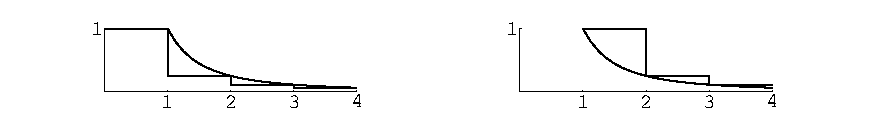
\includegraphics[width=0.8\textwidth]{fcv/series/bound}
      \caption{Upper and lower bounds on the sum.}
      \label{bound_series}
    \end{center}
  \end{figure}




\end{Example}

In general, we have
\[
\int_m^\infty a(x) \,\dd x \leq \sum_{n=m}^\infty a_n \leq a_m + \int_m^\infty a(x) \,\dd x.
\]
Thus we see that the sum converges or diverges with the integral.











\subsubsection{The Ratio Test.}
\index{ratio test}
\index{series!ratio test}
\index{convergence!ratio test}



\begin{Result}
  The series $\sum a_n$ converges absolutely if
  \[ 
  \lim_{n \to \infty} \left| \frac{a_{n+1}}{a_n} \right| < 1.
  \]
  If the limit is greater than unity, then the series diverges.  If the 
  limit is unity, the test fails.
\end{Result}


If the limit is greater than unity, then the terms are eventually increasing 
with $n$.  Since the terms do not vanish, the sum is divergent.
If the limit is less than unity, then there exists some $N$ such that 
\[ 
\left| \frac{a_{n+1}}{a_n} \right| \leq r < 1 \quad \mathrm{for all}\ n \geq N.
\]
From this we can show that $\sum_{n = 0}^\infty a_n$ is absolutely convergent by 
comparing it to the geometric series.
\begin{align*}
  \sum_{n=N}^\infty |a_n| &\leq |a_N| \sum_{n = 0}^\infty r^n 
  \\
  &= |a_N| \frac{1}{1 - r}
\end{align*}





\begin{Example}
  Consider the series,
  \[
  \sum_{n=1}^\infty \frac{\e^n}{n!}.
  \]
  We apply the ratio test to test for absolute convergence.
  \begin{align*}
    \lim_{n \to \infty} \left| \frac{a_{n+1}}{a_n} \right|
    &= \lim_{n \to \infty} \frac{\e^{n+1} n!}{\e^n (n + 1)!} 
    \\
    &= \lim_{n \to \infty} \frac{\e}{n + 1} 
    \\
    &= 0
  \end{align*}
  The series is absolutely convergent.
\end{Example}






\begin{Example}
  Consider the series,
  \[
  \sum_{n = 1}^\infty \frac{1}{n^2},
  \]
  which we know to be absolutely convergent.  We apply the ratio test.
  \begin{align*}
    \lim_{n \to \infty} \left| \frac{a_{n+1}}{a_n} \right|
    &= \lim_{n \to \infty} \frac{1/(n+1)^2}{1/n^2} 
    \\
    &= \lim_{n \to \infty} \frac{n^2}{n^2 + 2 n + 1} 
    \\
    &= \lim_{n \to \infty} \frac{1}{1 + 2 / n + 1 / n^2 } 
    \\
    &= 1
  \end{align*}
  The test fails to predict the absolute convergence of the series.
\end{Example}







\subsubsection{The Root Test.}
\index{root test}
\index{series!root test}
\index{convergence!root test}


\begin{Result}
  The series $\sum a_n$ converges absolutely if
  \[ 
  \lim_{n \to \infty} |a_n|^{1/n} < 1.
  \]
  If the limit is greater than unity, then the series diverges.  If the 
  limit is unity, the test fails.  More generally, we can test that
  \[
  \lim \sup |a_n|^{1/n} < 1.
  \]
\end{Result}




If the limit is greater than unity, then the terms in the series do not
vanish as $n \to \infty$.  This implies that the sum does not converge.
If the limit is less than unity, then there exists some $N$ such that 
\[ 
|a_n|^{1/n} \leq r < 1 \quad \mathrm{for all}\ n \geq N.
\]
We bound the tail of the series of $|a_n|$.
\begin{align*}
  \sum_{n=N}^\infty |a_n|
  &= \sum_{n=N}^\infty \left( |a_n|^{1/n} \right)^n 
  \\
  &\leq \sum_{n=N}^\infty r^n 
  \\
  &= \frac{r^N}{1-r}
\end{align*}
$\sum_{n = 0}^\infty a_n$ is absolutely convergent.






\begin{Example}
  Consider the series
  \[
  \sum_{n = 0}^\infty n^a b^n,
  \]
  where $a$ and $b$ are real constants.  We use the root test to check for 
  absolute convergence.
  \begin{gather*}
    \lim_{n \to \infty} \left| n^a b^n \right|^{1/n} < 1 
    \\
    |b| \lim_{n \to \infty} n^{a/n} < 1 
    \\
    |b| \exp \left( \lim_{n \to \infty} \frac{1 \ln n}{n} \right) < 1 
    \\
    |b| \e^0 < 1 
    \\
    |b| < 1
  \end{gather*}
  Thus we see that the series converges absolutely for $|b| < 1$.
  Note that the value of $a$ does not affect the absolute convergence.
\end{Example}







\begin{Example}
  Consider the absolutely convergent series,
  \[
  \sum_{n = 1}^\infty \frac{1}{n^2}.
  \]
  We aply the root test.
  \begin{align*}
    \lim_{n \to \infty} \left| a_n \right|^{1/n}
    &= \lim_{n \to \infty} \left| \frac{1}{n^2} \right|^{1/n} 
    \\
    &= \lim_{n \to \infty} n^{-2/n} 
    \\
    &= \lim_{n \to \infty} \e^{- \frac{2}{n} \ln n } 
    \\
    &= \e^0 
    \\
    &= 1
  \end{align*}
  It fails to predict the convergence of the series.
\end{Example}








\subsubsection{Raabe's Test}
\index{Raabe's test}
\index{series!Raabe's test}
\index{convergence!Raabe's test}



\begin{Result}
  The series $\sum a_n$ converges absolutely if
  \[ 
  \lim_{n \to \infty} n \left( 1 - \left| \frac{a_{n + 1}}{a_n} \right| \right) > 1.
  \]
  If the limit is less than unity, then the series diverges or converges 
  conditionally.  If the limit is unity, the test fails. 
\end{Result}

%% CONTINUE



\subsubsection{Gauss' Test}
\index{Gauss' test}
\index{series!Gauss' test}
\index{convergence!Gauss' test}

\begin{Result}
  Consider the series $\sum a_n$.  If
  \[
  \frac{a_{n+1}}{a_n} = 1 - \frac{L}{n} + \frac{b_n}{n^2}
  \]
  where $b_n$ is bounded then the series converges absolutely if 
  $L > 1$.  Otherwise the series diverges or converges conditionally.
\end{Result}




%% CONTINUE




%%============================================================================
\section{Uniform Convergence}
\label{sec_unif_conv}
\index{convergence!uniform}
\index{uniform convergence}



\paragraph{Continuous Functions.}
\index{continuous functions}
A function $f(z)$ is continuous in a closed domain if, given any
$\epsilon > 0$, there exists a $\delta > 0$ such that
$|f(z) - f(\zeta)| < \epsilon$ for all $|z-\zeta| < \delta$ in the domain.

An equivalent definition is that $f(z)$ is continuous in a closed domain
if 
\[
\lim_{\zeta \to z} f(\zeta) = f(z)
\]
for all $z$ in the domain.


\paragraph{Convergence.}
Consider a series in which the terms are functions of $z$, $\sum_{n = 0}^\infty a_n(z)$.
The series is convergent in a domain if the series converges 
for each point $z$ in the domain.  We can then define the function
$f(z) = \sum_{n = 0}^\infty a_n(z)$.  We can state the convergence criterion as:  
For any given $\epsilon > 0$ there exists a function $N(z)$ such that
\[ 
|f(z) - S_{N(z)}(z)| = \left|f(z) - \sum_{n=0}^{N(z)-1} a_n(z) \right| < \epsilon 
\]
for all $z$ in the domain.  Note that the rate of convergence, i.e. the 
number of terms, $N(z)$ required for for the absolute error to be less 
than $\epsilon$, is a function of $z$. 




\paragraph{Uniform Convergence.}
Consider a series $\sum_{n = 0}^\infty a_n(z)$ that is convergent in some domain.
If the rate of convergence is independent of $z$ then the series
is said to be uniformly convergent.  Stating this a little more mathematically,
the series is uniformly convergent in the domain if for any given $\epsilon
> 0$ there exists an $N$, independent of $z$, such that
\[ 
|f(z) - S_{N}(z)| = \left|f(z) - \sum_{n=1}^{N} a_n(z) \right| < \epsilon 
\]
for all $z$ in the domain.





%%-----------------------------------------------------------------------------
\subsection{Tests for Uniform Convergence}

\paragraph{Weierstrass M-test.}
\index{Weierstrass M-test}
The Weierstrass M-test
is useful in determining if a series is uniformly convergent.
The series $\sum_{n = 0}^\infty a_n(z)$ is uniformly and absolutely convergent in a 
domain if there exists a convergent series of positive terms
$\sum_{n = 0}^\infty M_n$ such that $|a_n(z)| \leq M_n$ for all $z$ in the domain.
This condition first implies that the series is absolutely convergent
for all $z$ in the domain.
The condition $|a_n(z)| \leq M_n$ also ensures that the rate of convergence is
independent of $z$, which is the criterion for uniform convergence.

Note that absolute convergence and uniform convergence are independent.
A series of functions may be absolutely convergent without being uniformly
convergent or vice versa.  The Weierstrass M-test is a sufficient but not a
necessary condition for uniform convergence.  The Weierstrass M-test can
succeed only if the series is uniformly and absolutely convergent.



\begin{Example}
  The series 
  \[ 
  f(x) = \sum_{n=1}^\infty \frac{\sin x}{n(n+1)} 
  \]
  is uniformly and absolutely convergent for all real $x$ because
  $|\frac{\sin x}{n (n+1)}| < \frac{1}{n^2}$ and $\sum_{n=1}^\infty \frac{1}{n^2}$
  converges.
\end{Example}






\paragraph{Dirichlet Test.}
Consider a sequence of monotone decreasing, positive constants ${c_n}$ with
limit zero.  If all the partial sums of $a_n(z)$ are bounded in some 
closed domain, that is
\[
\left| \sum_{n=1}^N a_n(z) \right| < \mathrm{constant}
\]
for all $N$, then $\sum_{n = 1}^\infty c_n a_n(z)$
is uniformly convergent in that closed domain.  Note that the Dirichlet
test does not imply that the series is absolutely convergent.




\begin{Example}
  \label{uniform_convergence_sin_nx_n}
  Consider the series,
  \[
  \sum_{n = 1}^\infty \frac{\sin(n x)}{n}.
  \]
  We cannot use the Weierstrass M-test to determine if the series is
  uniformly convergent on an interval.  While it is easy to bound the terms
  with $|\sin(n x)/n| \leq 1/n$, the sum
  \[
  \sum_{n = 1}^\infty \frac{1}{n}
  \]
  does not converge.  Thus we will try the Dirichlet test.  Consider the
  sum $\sum_{n=1}^{N-1} \sin(n x)$.  This sum can be evaluated in closed form. 
  (See Exercise~\ref{exercise sum sin nx}.)
  \[
  \sum_{n=1}^{N-1} \sin(n x) 
  = \begin{cases}
    0 &\mathrm{for}\ x = 2 \pi k 
    \\
    \frac{ \cos(x/2) - \cos((N-1/2) x)} { 2 \sin(x/2) } 
    &\mathrm{for}\ x \neq 2 \pi k
  \end{cases} 
  \]
  The partial sums have infinite discontinuities at $x = 2 \pi k$, 
  $k \in \mathbb{Z}$.
  The partial sums are bounded on any closed interval 
  that does not contain an integer multiple of $2 \pi$.
  By the Dirichlet test, the sum $\sum_{n = 1}^\infty \frac{\sin(n x)}{n}$ is uniformly
  convergent on any such closed interval.  The series may not be uniformly
  convergent in neighborhoods of $x = 2 k \pi$.  
\end{Example}








%%-----------------------------------------------------------------------------
\subsection{Uniform Convergence and Continuous Functions.}



Consider a series $f(z) = \sum_{n = 1}^\infty a_n(z)$ that is uniformly convergent
in some domain and whose terms $a_n(z)$ are continuous functions.  Since the
series is uniformly convergent, for any given $\epsilon > 0$ there exists
an $N$ such that $|R_N| < \epsilon$ for all $z$ in the
domain.

Since the finite sum $S_N$ is continuous, for that $\epsilon$
there exists a $\delta > 0$ such that 
$|S_N(z) - S_N(\zeta)| < \epsilon$ for all $\zeta$ in the domain satisfying $|z - \zeta| < \delta$.

We combine these two results to show that $f(z)$ is continuous.
\begin{align*}
  |f(z) - f(\zeta)|
  &= |S_N(z) + R_N(z) - S_N(\zeta) - R_N(\zeta)| 
  \\
  &\leq |S_N(z) - S_N(\zeta)| + |R_N(z)| + |R_N(\zeta)| 
  \\
  &< 3 \epsilon \quad \mathrm{for}\ |z - \zeta| < \delta
\end{align*}




\begin{Result}
  \label{unif_cont}
  A uniformly convergent series of continuous terms represents a continuous 
  function.
\end{Result}
\index{continuous functions}




\begin{Example}
  Again consider $\sum_{n = 1}^\infty \frac{\sin(n x)}{n}$.  In Example
  ~\ref{uniform_convergence_sin_nx_n} we showed that the convergence
  is uniform in any closed interval that does not contain an integer
  multiple of $2 \pi$.  In Figure~\ref{sinnx_n} is a plot of the first
  10 and then 50 terms in the series and finally the function to which
  the series converges.  We see that the function has jump
  discontinuities at $x = 2 k \pi$ and is continuous on any closed
  interval not containing one of those points.

  \begin{figure}[htb!]
    \begin{center}
      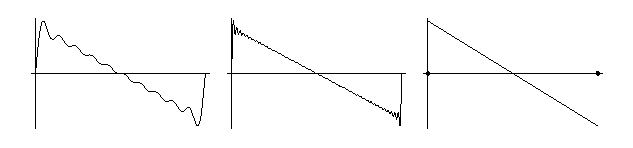
\includegraphics[width=\textwidth]{fcv/series/sinnx_n}
    \end{center}
    \caption{Ten, fifty and all the terms of the series.}
    \label{sinnx_n}
  \end{figure}

\end{Example}




%%============================================================================
%% CONTINUE: change the title
\section{Uniformly Convergent Power Series}
\index{power series!uniformly convergent}


\paragraph{Power Series.}
\index{power series!definition of}
Power series are series of the form
\[ 
\sum_{n = 0}^\infty a_n (z - z_0)^n.
\]



\paragraph{Domain of Convergence of a Power Series}
Consider the series $\sum_{n = 0}^{\infty} a_n z^n$.  Let the series converge
at some point $z_0$.  Then $|a_n z_0^n|$ is bounded by some constant $A$ for
all $n$, so
\[ 
|a_n z^n| = |a_n z_0^n| \left| \frac{z}{z_0} \right|^n 
< A \left| \frac{z}{z_0} \right|^n 
\]
This comparison test shows that the series converges absolutely for all $z$
satisfying $|z| < |z_0|$.

Suppose that the series diverges at some point $z_1$.  Then the series could
not converge for any $|z| > |z_1|$ since this would imply convergence at
$z_1$.  Thus there exists some circle in the $z$ plane such that the power
series converges absolutely inside the circle and diverges outside the circle.

\begin{Result}
  The domain of convergence of a power series is a circle in the 
  complex plane.
\end{Result}









\paragraph{Radius of Convergence of Power Series.}
Consider a power series
\[
f(z) = \sum_{n = 0}^\infty a_n z^n
\]
Applying the ratio test, we see that the series converges if
\begin{gather*}
  \lim_{n \to \infty} \frac{\left| a_{n+1} z^{n+1} \right|}{\left| a_n z^n \right|} < l 
  \\
  \lim_{n \to \infty} \frac{|a_{n+1}|}{|a_n|} |z| < 1 
  \\
  |z| < \lim_{n \to \infty} \frac{|a_n|}{|a_{n+1}|}
\end{gather*}





\begin{Result}
  \label{result ratio formula}
  \textbf{Ratio formula.}  
  The radius of convergence of the power series 
  \[
  \sum_{n = 0}^\infty a_n z^n
  \]
  is
  \[
  R = \lim_{n \to \infty} \frac{|a_n|}{|a_{n+1}|}
  \]
  when the limit exists.
\end{Result}
\index{power series!radius of convergence}






%%CONTINUE: Prove this.  Add examples.
\begin{Result}
  \label{result cauchy hadamard formula}
  \textbf{Cauchy-Hadamard formula.}  
  The radius of convergence of the power series:
  \[
  \sum_{n = 0}^\infty a_n z^n
  \]
  is
  \[
  R = \frac{ 1 }{ \lim \sup \sqrt[n]{ |a_n| } }.
  \]
\end{Result}




\paragraph{Absolute Convergence of Power Series.}
Consider a power series
\[ 
f(z) = \sum_{n = 0}^\infty a_n z^n 
\]
that converges for $z = z_0$.  Let $M$ be the value of the greatest term,
$a_n z_0^n$.  Consider any point $z$ such that $|z| < |z_0|$.
We can bound the residual of $\sum_{n = 0}^\infty |a_n z^n|$, 
\begin{align*}
  R_N(z)  &= \sum_{n=N}^\infty |a_n z^n| 
  \\
  &= \sum_{n=N}^\infty \left| \frac{a_n z^n}{a_n z_0^n} \right|  |a_n z_0^n| 
  \\
  &\leq M \sum_{n=N}^\infty \left|\frac{z}{z_0} \right|^n 
  \\
  \intertext{Since $|z / z_0| < 1$, this is a convergent geometric series.}
  &= M \left|\frac{z}{z_0}\right|^N \frac{1}{1 - |z/z_0|} 
  \\
  &\to 0 \quad \mathrm{as}\ N \to \infty
\end{align*}
Thus the power series is absolutely convergent for $|z| < |z_0|$. 



\begin{Result}
  If the power series $\sum_{n = 0}^\infty a_n z^n$ converges for $z = z_0$, then
  the series converges absolutely for $|z| < |z_0|$.
\end{Result}









\begin{Example}
  Find the radii of convergence of the following series.
  \begin{enumerate}
  \item 
    $\displaystyle \sum_{n = 1}^\infty n z^n$
  \item 
    $\displaystyle \sum_{n = 1}^\infty n! z^n$
  \item 
    $\displaystyle \sum_{n = 1}^\infty n! z^{n!}$
  \end{enumerate}

  \begin{enumerate}
    %%
  \item
    We apply the ratio test to determine the radius of convergence.
    \[
    R = \lim_{n \to \infty} \left| \frac{a_n}{a_{n+1}} \right| = \lim_{n \to \infty} \frac{n}{n + 1} = 1
    \]
    The series converges absolutely for $|z| < 1$.
    %%
  \item
    We apply the ratio test to the series.
    \begin{align*}
      R
      &= \lim_{n \to \infty} \left| \frac{n!}{(n+1)!} \right| 
      \\
      &= \lim_{n \to \infty} \frac{1}{n + 1} 
      \\
      &= 0
    \end{align*}
    The series has a vanishing radius of convergence. 
    It converges only for $z = 0$.
    %%
  \item
    Again we apply the ration test to determine the radius of convergence.
    \begin{gather*}
      \lim_{n \to \infty} \left| \frac{(n+1)! z^{(n+1)!}}{n! z^{n!}} \right| < 1 
      \\
      \lim_{n \to \infty} (n+1) |z|^{(n+1)! - n!} < 1 
      \\
      \lim_{n \to \infty} (n+1) |z|^{(n)n!} < 1 
      \\
      \lim_{n \to \infty} \left( \ln(n+1) + (n) n! \ln|z| \right) < 0 
      \\
      \ln |z| < \lim_{n \to \infty} \frac{- \ln(n + 1)}{(n) n!} 
      \\
      \ln |z| < 0 
      \\
      |z| < 1
    \end{gather*}
    The series converges absolutely for $|z| < 1$.

    Alternatively we could determine the radius of convergence of the
    series with the comparison test.
    \[
    \sum_{n = 1}^\infty \left| n! z^{n!} \right| \leq \sum_{n = 1}^\infty \left| n z^n \right|
    \]
    $\sum_{n = 1}^\infty n z^n$ has a radius of convergence of $1$.  Thus
    the series must have a radius of convergence of at least $1$.
    Note that if $|z| > 1$ then the terms in the series do not vanish
    as $n \to \infty$.  Thus the series must diverge for all $|z| \geq 1$.
    Again we see that the radius of convergence is $1$.
  \end{enumerate}
\end{Example}











\paragraph{Uniform Convergence of Power Series.}
Consider a power series $\sum_{n = 0}^\infty a_n z^n$ that converges in the 
disk $|z| < r_0$.  The sum converges absolutely for $z$ in the closed disk, 
$|z| \leq r < r_0$. Since $|a_n z^n| \leq |a_n r^n|$ and 
$\sum_{n = 0}^\infty |a_n r^n|$ converges, the power series is uniformly convergent
in $|z| \leq r < r_0$.



\begin{Result}
  If the power series $\sum_{n = 0}^\infty a_n z^n$ converges for $|z| < r_0$ then the
  series converges uniformly for $|z| \leq r < r_0$.
\end{Result}





\begin{Example} 
  \label{conv_unif_conv}
  \textbf{Convergence and Uniform Convergence.}
  Consider the series
  \[ 
  \log(1 - z) = -\sum_{n=1}^\infty \frac{z^n}{n}.
  \]
  This series converges for $|z| \leq 1, z \neq 1$.  
  Is the series uniformly convergent in this domain?  The residual after $N$ 
  terms $R_N$ is
  \[ 
  R_N(z) = \sum_{n=N+1}^\infty \frac{z^n}{n}.
  \]
  We can get a lower bound on the absolute value of the residual for real,
  positive $z$.
  \begin{align*}
    |R_N(x)| &= \sum_{n=N+1}^\infty \frac{x^n}{n} 
    \\
    &\leq \int_{N+1}^\infty \frac{x^\alpha}{\alpha}\,\dd \alpha 
    \\
    &= -\Ei((N+1) \ln x) 
  \end{align*}
  The exponential integral function, $\Ei(z)$, is defined
  \[ 
  \Ei(z) = - \int_{-z}^\infty \frac{\e^{-t}}{t}\,\dd t. 
  \]
  The exponential integral function is plotted in Figure~\ref{exp_int}.
  Since $\Ei(z)$ diverges as $z \to 0$, 
  by choosing $x$ sufficiently close to $1$ the residual can
  be made arbitrarily large.  Thus this series is not uniformly convergent
  in the domain $|z| \leq 1, z \neq 1$.
  The series is uniformly convergent for $|z| \leq r < 1$.

  \begin{center}
    \begin{figure}[htb!]
      \begin{center}
        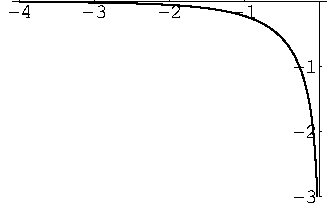
\includegraphics[width=0.35\textwidth]{fcv/series/exp_int}
      \end{center}
      \caption{The exponential integral function.}
      \label{exp_int}
    \end{figure}
  \end{center}

\end{Example}








\paragraph{Analyticity.}
Recall that a sufficient condition for the analyticity of a function $f(z)$
in a domain is that $\oint_C f(z)\,\dd z = 0$ for all simple, closed
contours in the domain.

Consider a power series $f(z) = \sum_{n = 0}^\infty a_n z^n$ that is uniformly
convergent in $|z| \leq r$.  If $C$ is any simple, closed contour in the
domain then $\oint_C f(z)\,\dd z$ exists.  Expanding $f(z)$ into a finite
series and a residual,
\[ 
\oint_C f(z)\,\dd z = \oint_C \left( S_N(z) + R_N(z) \right)\,\dd z.
\]
Since the series is uniformly convergent, for any given $\epsilon > 0$ there
exists an $N_\epsilon$ such that $|R_{N_\epsilon}| < \epsilon$ for all $z$
in $|z| \leq r$. Let $L$ be the length of the contour $C$.
\[ 
\left| \oint_C R_{N_\epsilon}(z)\,\dd z \right| \leq L \epsilon \to 0 \quad \mathrm{as}\ N_\epsilon \to \infty
\]
\begin{align*}
  \oint_C f(z)\,\dd z
  &=\lim_{N \to \infty} \oint_C \left( \sum_{n=0}^{N-1} a_n z^n + R_N(z) \right)\,\dd z 
  \\
  &= \oint_C \sum_{n = 0}^\infty a_n z^n 
  \\
  &= \sum_{n = 0}^\infty a_n \oint_C z^n\,\dd z 
  \\
  &= 0
\end{align*}
Thus $f(z)$ is analytic for $|z| < r$.



\begin{Result}
  A power series is analytic in its domain of uniform convergence.
\end{Result}








%%============================================================================
\section{Integration and Differentiation of Power Series}
\index{power series!integration of}
\index{power series!differentiation of}



Consider a power series $f(z) = \sum_{n = 0}^\infty a_n z^n$ that is convergent in the 
disk $|z| < r_0$.  Let $C$ be any contour of finite length $L$
lying entirely within the closed domain $|z| \leq r < r_0$.  
The integral of $f(z)$ along $C$ is
\[
\int_C f(z)\,\dd z = \int_C (S_N(z) + R_N(z))\,\dd z.
\]
Since the series is uniformly convergent in the closed disk, 
for any given $\epsilon > 0$, there exists an $N_\epsilon$ such that
\[ 
|R_{N_\epsilon}(z)| < \epsilon \quad \mathrm{for all}\ |z| \leq r.
\]
We bound the absolute value of the integral of $R_{N_\epsilon}(z)$.
\begin{align*}
  \left| \int_C R_{N_\epsilon}(z)\,\dd z \right|
  &\leq \int_C |R_{N_\epsilon}(z)|\,\dd z 
  \\
  &< \epsilon L 
  \\
  &\to 0 \quad \mathrm{as}\ N_\epsilon \to \infty
\end{align*}
Thus
\begin{align*}
  \int_C f(z)\,\dd z
  &= \lim_{N \to \infty} \int_C \sum_{n=0}^N a_n z^n\,\dd z 
  \\
  &= \lim_{N \to \infty} \sum_{n=0}^N a_n \int_C z^n\,\dd z 
  \\
  &= \sum_{n = 0}^\infty a_n \int_C z^n\,\dd z
\end{align*}












\begin{Result}
  If $C$ is a contour lying in the domain of uniform convergence of the
  power series $\sum_{n = 0}^\infty a_n z^n$ then
  \[ 
  \int_C \sum_{n = 0}^\infty a_n z^n \,\dd z = \sum_{n = 0}^\infty a_n \int_C z^n\,\dd z.
  \]
\end{Result}




In the domain of uniform convergence of a series we can interchange the
order of summation and a limit process.  That is,
\[ 
\lim_{z \to z_0} \sum_{n = 0}^\infty a_n(z) = \sum_{n = 0}^\infty \lim_{z \to z_0} a_n(z).
\]
We can do this because the rate of convergence does not depend on $z$.
Since differentiation is a limit process,
\[ 
\frac{\dd}{\dd z} f(z) = \lim_{h \to 0} \frac{f(z+h) - f(z)}{h},
\]
we would expect that we could differentiate a uniformly convergent series. 

Since we showed that a uniformly convergent power series is equal to an 
analytic function, we can differentiate a power series in its domain of 
uniform convergence.



\begin{Result}
  Power series can be differentiated in their domain of uniform convergence.
  \[ 
  \frac{\dd}{\dd z} \sum_{n = 0}^\infty a_n z^n = \sum_{n = 0}^\infty (n + 1) a_{n+1} z^n. 
  \]
\end{Result}








\begin{Example} \textbf{Differentiating a Series.}
  Consider the series from Example~\ref{conv_unif_conv}.
  \[ 
  \log(1 - z) = - \sum_{n=1}^\infty \frac{z^n}{n}
  \]
  We differentiate this to obtain the geometric series.
  \begin{gather*}
    - \frac{1}{1 - z} = - \sum_{n=1}^\infty z^{n-1} 
    \\
    \frac{1}{1 - z} = \sum_{n = 0}^\infty z^n
  \end{gather*}
  The geometric series is convergent for  
  $|z| < 1$ and uniformly convergent for $|z| \leq r < 1$.  Note that the 
  domain of convergence is different than the series for $\log(1 - z)$.
  The geometric series does not converge for $|z| = 1, z \neq 1$. 
  However, the domain of uniform convergence has remained the same.
\end{Example}









%%============================================================================
\section{Taylor Series}
\index{Taylor series}



\begin{Result}
  \label{result taylor theorem}
  \textbf{Taylor's Theorem.}
  Let $f(z)$ be a function that is single-valued and analytic in 
  $|z - z_0| < R$.  For all $z$ in this open disk, $f(z)$ has the 
  convergent Taylor series
  \begin{equation}
    \label{eqn_taylors_theorem1} 
    f(z) = \sum_{n = 0}^\infty \frac{f^{(n)}(z_0)}{n!} (z - z_0)^n.
  \end{equation}
  We can also write this as 
  \begin{equation}
    \label{eqn_taylors_theorem2}
    f(z) = \sum_{n = 0}^\infty a_n (z - z_0)^n, \quad 
    a_n = \frac{ f^{(n)}(z_0) }{ n! }
    = \frac{ 1 }{ \imath 2 \pi } \oint_C \frac{ f(z) }{ (z - z_0)^{n+1} } \,\dd z,
  \end{equation}
  where $C$ is a simple, positive, closed contour in $0 < |z - z_0| < R$ 
  that goes once around the point $z_0$.
\end{Result}





\paragraph{Proof of Taylor's Theorem.}
Let's see why Result~\ref{result taylor theorem} is true.  
Consider a function $f(z)$ that is analytic
in $|z| < R$.  (Considering $z_0 \neq 0$ is only trivially more general as
we can introduce the change of variables $\zeta = z - z_0$.)  According 
to Cauchy's Integral Formula, (Result~\ref{cauchy_formula}),
\begin{equation}
  \label{eqn_cauchy_formula_z_zeta} 
  f(z) = \frac{1}{\imath 2 \pi} \oint_C \frac{f(\zeta)}{\zeta-z}\,\dd \zeta,
\end{equation}
where $C$ is a positive, simple, closed contour in $0 < |\zeta - z| < R$ that
goes once around $z$.  We take this contour to be the circle about the
origin of radius $r$ where $|z| < r < R$.
(See Figure~\ref{taylor_circles}.)



\begin{figure}[htb!]
  \begin{center}
    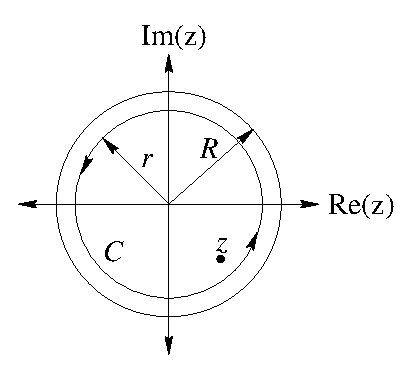
\includegraphics[width=0.3\textwidth]{fcv/series/taylor_circles}
    \caption{Graph of the domain of convergence and the contour 
      of integration.}
    \label{taylor_circles}
  \end{center}
\end{figure}


We expand $\frac{1}{\zeta - z}$ in a geometric series,
\begin{align*}
  \frac{1}{\zeta - z} 
  &= \frac{1/\zeta}{1 - z/\zeta} 
  \\
  &= \frac{1}{\zeta} \sum_{n = 0}^\infty \left( \frac{ z }{ \zeta } \right)^n,
  \quad \mathrm{for}\ |z| < |\zeta| 
  \\
  &= \sum_{n = 0}^\infty \frac{ z^n }{ \zeta^{n+1} }, \quad \mathrm{for}\ |z| < |\zeta|
\end{align*}
We substitute this series into Equation~\ref{eqn_cauchy_formula_z_zeta}.
\begin{align*}
  f(z)    
  &= \frac{1}{\imath 2 \pi} \oint_C \left( 
    \sum_{n = 0}^\infty \frac{ f(\zeta) z^n }{ \zeta^{n+1} } \right)\,\dd \zeta 
  \\
  \intertext{The series converges uniformly so we can interchange 
    integration and summation.}
  &= \sum_{n = 0}^\infty \frac{z^n}{\imath 2 \pi} \oint_C \frac{ f(\zeta) }{ \zeta^{n+1} }\,\dd \zeta \\
  \intertext{Now we have derived Equation~\ref{eqn_taylors_theorem2}.
    To obtain Equation~\ref{eqn_taylors_theorem1}, we apply Cauchy's Integral 
    Formula.}
  &= \sum_{n = 0}^\infty \frac{f^{(n)}(0)}{n!} z^n
\end{align*}

There is a table of some commonly encountered Taylor series in Appendix
~\ref{table_of_taylor_series}.





\begin{Example}
  Consider the Taylor series expansion of $1/(1 - z)$ about $z = 0$.
  Previously, we showed that this function is the sum of the geometric series
  $\sum_{n = 0}^\infty z^n$ and we used the ratio test to show that the series 
  converged absolutely for $|z| < 1$.  Now we find the series using
  Taylor's theorem.  Since the nearest singularity of the function is at 
  $z = 1$, the radius of convergence of the series is $1$.
  The coefficients in the series are
  \begin{align*}
    a_n     
    &= \frac{1}{n!} \left[ \frac{\dd^n}{\dd z^n} \frac{1}{1 - z} \right]_{z=0} 
    \\
    &= \frac{1}{n!} \left[ \frac{n!}{(1 - z)^n} \right]_{z=0} 
    \\
    &= 1
  \end{align*}
  Thus we have
  \[
  \frac{1}{1-z} = \sum_{n = 0}^\infty z^n , \qquad \mathrm{for}\ |z| < 1.
  \]
\end{Example}











%%---------------------------------------------------------------------------
\subsection{Newton's Binomial Formula.}




\begin{Result}
  For all $|z| < 1$, $a$ complex:
  \[ 
  (1 + z)^a = 1 + \binom{a}{1} z + \binom{a}{2} z^2 + \binom{a}{3} z^3 + \cdots 
  \]
  where
  \[ 
  \binom{a}{r} = \frac{a (a-1) (a-2)\cdots(a-r+1)}{r!}. 
  \]
  If $a$ is complex, then the expansion is of the principle branch of
  $(1 + z)^a$.  We define
  \[
  \binom{r}{0} = 1, \quad \binom{0}{r} = 0, \quad \mathrm{for}\ r \neq 0,
  \qquad \binom{0}{0} = 1.
  \]
\end{Result}






\begin{Example}
  Evaluate $ \lim_{n \to \infty} (1 + 1/n)^n$.

  First we expand $(1 + 1/n)^n$ using Newton's binomial formula.
  \begin{align*}
    \lim_{n \to \infty} \left(1 + \frac{1}{n} \right)^n 
    &= \lim_{n \to \infty} \left( 1 + \binom{n}{1} \frac{1}{n} +
      \binom{n}{2} \frac{1}{n^2} + \binom{n}{3} \frac{1}{n^3} + \cdots  \right) 
    \\
    &= \lim_{n \to \infty} \left( 1 + 1 + \frac{n (n-1)}{2! n^2} +
      \frac{n (n-1) (n-2)}{3! n^3} + \cdots \right) 
    \\
    &= \left( 1 + 1 + \frac{1}{2!} + \frac{1}{3!} + \cdots \right) 
    \\
    \intertext{We recognize this as the Taylor series expansion of $\e^1$.}
    &= \e
  \end{align*}
  We can also evaluate the limit using L'Hospital's rule.
  \begin{align*}
    \ln \left(\lim_{x \to \infty} \left(1 + \frac{1}{x} \right)^x \right)
    &= \lim_{x \to \infty} \ln \left( \left( 1 + \frac{1}{x} \right)^x \right) 
    \\
    &= \lim_{x \to \infty} x \ln\left( 1 + \frac{1}{x} \right) 
    \\
    &= \lim_{x \to \infty} \frac{\ln(1 + 1/x)}{1/x}  
    \\
    &= \lim_{x \to \infty} \frac{\frac{-1/x^2}{1 + 1/x}}{-1/x^2} 
    \\
    &= 1
  \end{align*}
  \[
  \lim_{x \to \infty} \left(1 + \frac{1}{x} \right)^x = \e
  \]
\end{Example}





\begin{Example}
  Find the Taylor series expansion of $1/(1 + z)$ about $z = 0$.

  For $|z| < 1$,
  \begin{align*}
    \frac{1}{1 + z} &= 1 + \binom{-1}{1} z + \binom{-1}{2} z^2 +
    \binom{-1}{3} z^3 + \cdots 
    \\
    &= 1 + (-1)^1 z + (-1)^2 z^2 + (-1)^3 z^3 + \cdots 
    \\
    &= 1 - z + z^2 - z^3 + \cdots
  \end{align*}
\end{Example}






\begin{Example}
  Find the first few terms in the Taylor series expansion of
  \[
  \frac{1}{\sqrt{z^2 + 5 z + 6}}
  \]
  about the origin.

  We factor the denominator and then apply Newton's binomial formula.
  \begin{align*}
    \frac{1}{\sqrt{z^2 + 5 z + 6}}
    &= \frac{1}{\sqrt{z + 3}} \frac{1}{\sqrt{z + 2}} 
    \\
    &= \frac{1}{\sqrt{3} \sqrt{1 + z/3}} \frac{1}{\sqrt{2} \sqrt{1+z/2}} 
    \\
    &= \frac{1}{\sqrt{6}} \left( 1 + \binom{-1/2}{1} \frac{z}{3}
      + \binom{-1/2}{2} \left(\frac{z}{3}\right)^2 + \cdots \right)
    \left( 1 + \binom{-1/2}{1} \frac{z}{2}
      + \binom{-1/2}{2} \left(\frac{z}{2}\right)^2 + \cdots \right)
    \\
    &= \frac{1}{\sqrt{6}} \left( 1 - \frac{z}{6} + \frac{z^2}{24} + \cdots
    \right)
    \left( 1 - \frac{z}{4} + \frac{3 z^2}{32} + \cdots \right) 
    \\
    &= \frac{1}{\sqrt{6}} \left( 1 - \frac{5}{12} z + \frac{17}{96} z^2
      + \cdots \right)
  \end{align*}
\end{Example}













%%===========================================================================
\section{Laurent Series}
\index{Laurent series}

\begin{Result}
  Let $f(z)$ be single-valued and analytic in the annulus 
  $R_1 < |z - z_0| < R_2$.  For points in the annulus, the function
  has the convergent Laurent series
  \[ 
  f(z) = \sum_{n = -\infty}^\infty a_n z^n,
  \]
  where 
  \[ 
  a_n = \frac{1}{\imath 2 \pi} \oint_C \frac{f(z)}{(z - z_0)^{n+1}}\,\dd z 
  \]
  and $C$ is a positively oriented, closed contour around $z_0$ 
  lying in the annulus.
\end{Result}



To derive this result, consider a function $f(\zeta)$ that is analytic in the 
annulus $R_1 < |\zeta| < R_2$.  Consider any point $z$ in the annulus.
Let $C_1$ be a circle of radius $r_1$ with
$R_1 < r_1 < |z|$.  Let $C_2$ be a circle of radius $r_2$ with
$|z| < r_2 < R_2$. 
Let $C_z$ be a circle around $z$, lying entirely between $C_1$ and $C_2$.
(See Figure~\ref{laur_cont} for an illustration.)

Consider the integral of $\frac{f(\zeta)}{\zeta - z}$ around the $C_2$ contour.
Since the the only singularities of $\frac{f(\zeta)}{\zeta - z}$ occur at
$\zeta = z$ and at points outside the annulus,
\[ 
\oint_{C_2} \frac{f(\zeta)}{\zeta - z}\,\dd \zeta 
= \oint_{C_z} \frac{f(\zeta)}{\zeta - z}\,\dd \zeta
+ \oint_{C_1} \frac{f(\zeta)}{\zeta - z}\,\dd \zeta. 
\]
By Cauchy's Integral Formula, the integral around $C_z$ is
\[ 
\oint_{C_z} \frac{f(\zeta)}{\zeta - z}\,\dd \zeta = \imath 2 \pi f(z).
\]
This gives us an expression for $f(z)$.
\begin{equation}
  \label{eqn_fz_int_int} 
  f(z) = \frac{1}{\imath 2 \pi} \oint_{C_2} \frac{f(\zeta)}{\zeta - z}\,\dd \zeta 
  - \frac{1}{\imath 2 \pi} \oint_{C_1} \frac{f(\zeta)}{\zeta - z}\,\dd \zeta
\end{equation}

On the $C_2$ contour, $|z| < |\zeta|$.  Thus 
\begin{align*}
  \frac{1}{\zeta - z}
  &= \frac{1/\zeta}{1 - z/\zeta} 
  \\
  &= \frac{1}{\zeta} \sum_{n = 0}^\infty \left( \frac{z}{\zeta} \right)^n,
  \quad \mathrm{for}\ |z| < |\zeta| 
  \\
  &= \sum_{n = 0}^\infty \frac{ z^n }{ \zeta^{n+1} }, \quad \mathrm{for}\ |z| < |\zeta|
\end{align*}
On the $C_1$ contour, $|\zeta| < |z|$.  Thus
\begin{align*}
  - \frac{1}{\zeta - z} 
  &= \frac{1/z}{1 - \zeta/z} 
  \\
  &= \frac{1}{z} \sum_{n = 0}^\infty \left( \frac{\zeta}{z} \right)^n, 
  \quad \mathrm{for}\ |\zeta| < |z| 
  \\
  &= \sum_{n = 0}^\infty \frac{\zeta^n}{z^{n+1}}, \quad \mathrm{for}\ |\zeta| < |z| 
  \\
  &= \sum_{n = -\infty}^{-1} \frac{ z^n }{ \zeta^{n+1} }, \quad \mathrm{for}\ |\zeta| < |z| 
\end{align*}

We substitute these geometric series into Equation~\ref{eqn_fz_int_int}.
\begin{gather*}
  f(z) = \frac{1}{\imath 2 \pi} \oint_{C_2} \left( \sum_{n = 0}^\infty 
    \frac{ f(\zeta) z^n }{ \zeta^{n+1} } \right)\,\dd \zeta 
  + \frac{1}{\imath 2 \pi} \oint_{C_1} \left( \sum_{n = -\infty}^{-1} 
    \frac{ f(\zeta) z^n }{ \zeta^{n+1} } \right)\,\dd \zeta 
  \\
  \intertext{Since the sums converge uniformly, we can interchange the
    order of integration and summation.}
  f(z) = \frac{1}{\imath 2 \pi} \sum_{n = 0}^\infty \oint_{C_2} \frac{ f(\zeta) z^n }{ \zeta^{n+1} }\,\dd \zeta 
  + \frac{1}{\imath 2 \pi} \sum_{n = -\infty}^{-1} \oint_{C_1} \frac{ f(\zeta) z^n }{ \zeta^{n+1} }\,\dd \zeta 
\end{gather*}
Since the only singularities of the integrands lie outside of the annulus,
the $C_1$ and $C_2$ contours can be deformed to any positive, closed 
contour $C$ that lies in the annulus and encloses the origin.
(See Figure~\ref{laur_cont}.) 
Finally, we combine the two integrals to obtain the desired result.
\[
f(z) = \sum_{n = -\infty}^\infty \frac{1}{\imath 2 \pi} \left( \oint_{C} \frac{ f(\zeta) }{ \zeta^{n+1} }\,\dd \zeta 
\right) z^n
\]
For the case of arbitrary $z_0$, simply make the transformation
$z \to z - z_0$.

\begin{figure}[htb!]
  \begin{center}
    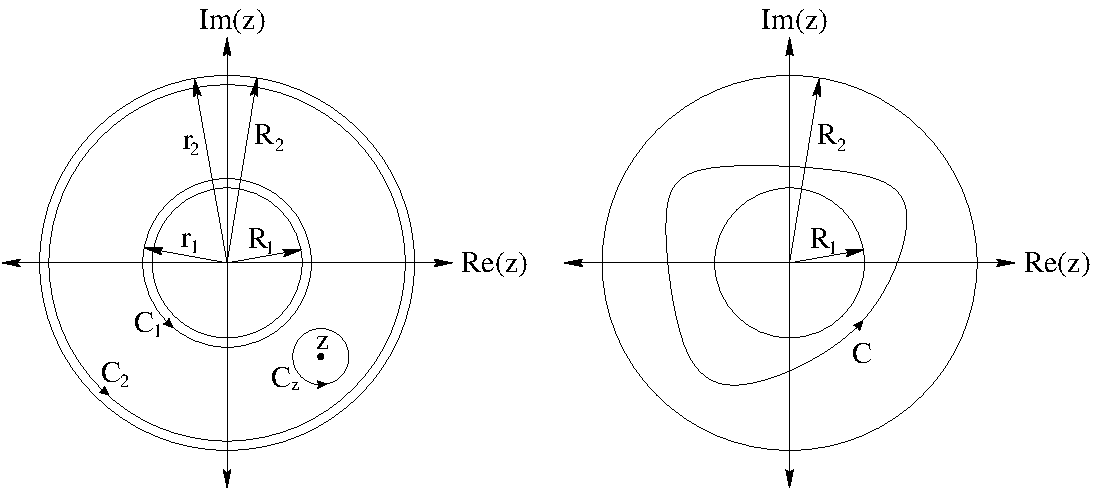
\includegraphics[width=0.8\textwidth]{fcv/series/laur_cont}
  \end{center}
  \caption{Contours for a Laurent expansion in an annulus.}
  \label{laur_cont}
\end{figure}












\begin{Example}
  Find the Laurent series expansions of $1/(1 + z)$.

  For $|z| < 1$,
  \begin{align*}
    \frac{1}{1 + z} &= 1 + \binom{-1}{1} z + \binom{-1}{2} z^2 
    + \binom{-1}{3} z^3 + \cdots 
    \\
    &= 1 + (-1)^1 z + (-1)^2 z^2 + (-1)^3 z^3 + \cdots 
    \\
    &= 1 - z + z^2 - z^3 + \cdots
  \end{align*}

  For $|z| > 1$,
  \begin{align*}
    \frac{1}{1 + z} 
    &= \frac{1/z}{1 + 1/z} 
    \\
    &= \frac{1}{z} \left( 1 + \binom{-1}{1} z^{-1} + \binom{-1}{2} z^{-2}
      + \cdots \right)  
    \\
    &= z^{-1} - z^{-2} + z^{-3} - \cdots
  \end{align*}
\end{Example}









\raggedbottom
%%============================================================================
\exercises{
\pagebreak
\flushbottom
\section{Exercises}




%%-----------------------------------------------------------------------------
\begin{large}
  \noindent
  \textbf{Series of Constants}
\end{large}


\begin{Exercise}
  \label{exercise lim an = 0 necessary series convergence}
  Show that if $\sum a_n$ converges then $\lim_{n \to \infty} a_n = 0$.
  That is, $\lim_{n \to \infty} a_n = 0$ is a necessary 
  condition for the convergence of the series.

  \hintsolution{lim an = 0 necessary series convergence}
\end{Exercise}


\begin{Exercise}
  \label{exercise series true false}
  Answer the following questions \textit{true} or \textit{false}.  
  Justify your answers.
  \begin{enumerate}
  \item
    There exists a sequence which converges to both $1$ and $-1$.
  \item
    There exists a sequence $\{ a_n \}$ such that $a_n > 1$ for all $n$ and 
    $\lim_{n \to \infty} a_n = 1$.
  \item
    There exists a divergent geometric series whose terms converge.
  \item
    There exists a sequence whose even terms are greater than $1$,
    whose odd terms are less than $1$ and that converges to $1$.
  \item
    There exists a divergent series of non-negative terms,
    $\sum_{n = 0}^\infty a_n$, such that $a_n < (1/2)^n$.
  \item
    There exists a convergent sequence, $\{ a_n \}$, such that 
    $\lim_{n \to \infty} (a_{n+1} - a_n) \neq 0$.
  \item
    There exists a divergent sequence, $\{ a_n \}$, such that
    $\lim_{n \to \infty} |a_n| = 2$.
  \item
    There exists divergent series, $\sum a_n$ and $\sum b_n$, such that
    $\sum (a_n + b_n)$ is convergent.
  \item
    There exists 2 different series of nonzero terms that have the same sum.
  \item
    There exists a series of nonzero terms that converges to zero.
  \item
    There exists a series with an infinite number of non-real terms which
    converges to a real number.
  \item
    There exists a convergent series $\sum a_n$ with 
    $\lim_{n \to \infty} |a_{n+1}/a_n| = 1$.
  \item
    There exists a divergent series $\sum a_n$ with 
    $\lim_{n \to \infty} |a_{n+1}/a_n| = 1$.
  \item
    There exists a convergent series $\sum a_n$ with 
    $\lim_{n \to \infty} \sqrt[n]{|a_n|} = 1$.
  \item
    There exists a divergent series $\sum a_n$ with 
    $\lim_{n \to \infty} \sqrt[n]{|a_n|} = 1$.
  \item
    There exists a convergent series of non-negative terms, $\sum a_n$,
    for which $\sum a_n^2$ diverges.
  \item
    There exists a convergent series of non-negative terms, $\sum a_n$,
    for which $\sum \sqrt{a_n}$ diverges.
  \item
    There exists a convergent series, $\sum a_n$,
    for which $\sum |a_n|$ diverges.
  \item
    There exists a power series $\sum a_n (z - z_0)^n$ which converges for 
    $z = 0$ and $z = 3$ but diverges for $z = 2$.
  \item
    There exists a power series $\sum a_n (z - z_0)^n$ which converges for 
    $z = 0$ and $z = \imath 2$ but diverges for $z = 2$.
  \end{enumerate}

  \hintsolution{series true false}
\end{Exercise}



\begin{Exercise}
  \label{exercise convergence 1/ ln(nn)}
  Determine if the following series converge.
  \begin{enumerate}
  \item
    $\displaystyle \sum_{n=2}^\infty \frac{1}{n \ln(n)}$
  \item
    $\displaystyle \sum_{n=2}^\infty \frac{1}{\ln \left( n^n \right)}$
  \item
    $\displaystyle \sum_{n=2}^\infty \ln \sqrt[n]{\ln n}$
  \item
    $\displaystyle \sum_{n=10}^\infty \frac{1}{ n (\ln n) (\ln(\ln n)) }$
  \item
    $\displaystyle \sum_{n=1}^\infty \frac{ \ln \left( 2^n \right) }
    { \ln \left( 3^n \right) + 1 }$
  \item
    $\displaystyle \sum_{n=0}^\infty \frac{1}{\ln(n + 20)}$
  \item
    $\displaystyle \sum_{n=0}^\infty \frac{4^n + 1}{3^n - 2}$
  \item
    $\displaystyle \sum_{n=0}^\infty (\Log_\pi 2)^n$
  \item
    $\displaystyle \sum_{n=2}^\infty \frac{n^2 - 1}{n^4 - 1}$
  \item
    $\displaystyle \sum_{n=2}^\infty \frac{n^2}{(\ln n)^n}$
  \item
    $\displaystyle \sum_{n=2}^\infty (-1)^n \ln \left( \frac{1}{n} \right)$
  \item
    $\displaystyle \sum_{n=2}^\infty \frac{ (n!)^2 }{ (2 n)! }$
  \item
    $\displaystyle \sum_{n=2}^\infty \frac{3^n + 4^n + 5}{5^n - 4^n - 3}$
  \item
    $\displaystyle \sum_{n=2}^\infty \frac{ n! }{ (\ln n)^n }$
  \item
    $\displaystyle \sum_{n=2}^\infty \frac{\e^n}{\ln(n!)}$
  \item
    $\displaystyle \sum_{n=1}^\infty \frac{ (n!)^2 }{ (n^2)! }$
  \item
    $\displaystyle \sum_{n=1}^\infty \frac{n^8 + 4 n^4 + 8}{3 n^9 - n^5 + 9 n}$
  \item
    $\displaystyle \sum_{n=1}^\infty \left( \frac{1}{n} - \frac{1}{n+1} \right)$
  \item
    $\displaystyle \sum_{n=1}^\infty \frac{\cos( n \pi )}{n}$
  \item
    $\displaystyle \sum_{n=2}^\infty \frac{ \ln n }{ n^{11/10} }$
  \end{enumerate}

  \hintsolution{convergence 1/ ln(nn)}
\end{Exercise}


\begin{Exercise}[mathematica/fcv/series/constants.nb]
  \label{exercise alternating harmonic series}
  Show that the alternating harmonic series,
  \[
  \sum_{n = 1}^\infty \frac{(-1)^{n+1}}{n} = 1 - \frac{1}{2} + \frac{1}{3} - \frac{1}{4}
  + \cdots,
  \]
  is convergent.

  \hintsolution{alternating harmonic series}
\end{Exercise}



\begin{Exercise}[mathematica/fcv/series/constants.nb]
  \label{exercise divergent harmonic series}
  Show that the series
  \[
  \sum_{n = 1}^\infty \frac{1}{n}
  \]
  is divergent with the Cauchy convergence criterion.

  \hintsolution{divergent harmonic series}
\end{Exercise}



%% Rearrange alternating harmonic series.
\begin{Exercise}
  \label{exercise rearrange alternating harmonic series}
  The alternating harmonic series has the sum:
  \[
  \sum_{n = 1}^\infty \frac{(-1)^n}{n} = \ln(2).
  \]
  Show that the terms in this series can be rearranged to sum to $\pi$.

  \hintsolution{rearrange alternating harmonic series}
\end{Exercise}




%%
\begin{Exercise}[mathematica/fcv/series/constants.nb]
  \label{exercise sum n!/n^n}
  Is the series,
  \[
  \sum_{n = 1}^\infty \frac{n!}{n^n},
  \]
  convergent?

  \hintsolution{sum n!/n^n}
\end{Exercise}

%% CONTINUE: solve the rest of the exercises in Mathematica.


%% convergence/divergence of the harmonic series.
\begin{Exercise}
  \label{exercise harmonic series}
  \index{harmonic series}
  Show that the harmonic series,
  \[ 
  \sum_{n=1}^\infty \frac{1}{n^\alpha} = 1 + \frac{1}{2^\alpha} + \frac{1}{3^\alpha} + \cdots,
  \]
  converges for $\alpha > 1$ and diverges for $\alpha \leq 1$.

  \hintsolution{harmonic series}
\end{Exercise}



%% Evaluate \sum_{n=1}^{N-1} \sin(n x)
\begin{Exercise}
  \label{exercise sum sin nx}
  Evaluate $\sum_{n=1}^{N-1} \sin(n x)$.

  \hintsolution{sum sin nx}
\end{Exercise}


\begin{Exercise}
  \label{exercise sum k z^k}
  Evaluate
  \[
  \sum_{k=1}^n k z^k \quad \mathrm{and} \quad \sum_{k=1}^n k^2 z^k
  \]
  for $z \neq 1$.

  \hintsolution{sum k z^k}
\end{Exercise}


\begin{Exercise}
  \label{exercise sum rational alternate geometric}
  Which of the following series converge?  Find the sum of those that do.
  \begin{enumerate}
  \item 
    $\displaystyle \frac{1}{2} + \frac{1}{6} + \frac{1}{12}
    + \frac{1}{20} + \cdots$
  \item 
    $\displaystyle 1 + (-1) + 1 + (-1) + \cdots$
  \item 
    $\displaystyle \sum_{n = 1}^\infty \frac{1}{2^{n-1}} \frac{1}{3^n} \frac{1}{5^{n+1}}$
  \end{enumerate}

  \hintsolution{sum rational alternate geometric}
\end{Exercise}








\begin{Exercise}
  \label{exercise sum sum 1/2 k}
  Evaluate the following sum.
  \[
  \sum_{k_1 = 0}^\infty \sum_{k_2 = k_1}^\infty \cdots \sum_{k_n = k_{n-1}}^\infty \frac{1}{2^{k_n}}
  \]

  \hintsolution{sum sum 1/2 k}
\end{Exercise}



%%-----------------------------------------------------------------------------
\begin{large}
  \noindent
  \textbf{Uniform Convergence}
\end{large}



%%-----------------------------------------------------------------------------
\begin{large}
  \noindent
  \textbf{Uniformly Convergent Power Series}
\end{large}


\begin{Exercise}
  \label{exercise convergence zn / (z+3)n}
  Determine the domain of convergence of the following series.
  \begin{enumerate}
  \item
    $\displaystyle \sum_{n=0}^\infty \frac{z^n}{(z + 3)^n}$
  \item
    $\displaystyle \sum_{n=2}^\infty \frac{\Log z}{\ln n}$
  \item
    $\displaystyle \sum_{n=1}^\infty \frac{z}{n}$
  \item
    $\displaystyle \sum_{n=1}^\infty \frac{(z + 2)^2}{n^2}$
  \item
    $\displaystyle \sum_{n=1}^\infty \frac{(z - \e)^n}{n^n}$
  \item
    $\displaystyle \sum_{n=1}^\infty \frac{z^{2n}}{2^{n z}}$
  \item
    $\displaystyle \sum_{n=0}^\infty \frac{z^{n!}}{(n!)^2}$
  \item
    $\displaystyle \sum_{n=0}^\infty \frac{z^{\ln(n!)}}{n!}$
  \item
    $\displaystyle \sum_{n=0}^\infty \frac{ (z - \pi)^{2 n + 1} n^\pi }{ n! }$
  \item
    $\displaystyle \sum_{n=0}^\infty \frac{ \ln n }{ z^n }$
  \end{enumerate}

  \hintsolution{convergence zn / (z+3)n}
\end{Exercise}




%% \sum_{n = 1}^\infty \frac{n}{2^n} (z - i)^n
\begin{Exercise}
  \label{exercise convergence n/2^n (z-i)^n}
  Find the circle of convergence of the following series.
  \begin{enumerate}
  \item $\displaystyle z + (\alpha - \beta) \frac{z^2}{2!}
    + (\alpha - \beta) (\alpha - 2 \beta) \frac{z^3}{3!}
    + (\alpha - \beta) (\alpha - 2 \beta)(\alpha - 3 \beta) \frac{z^4}{4!} + \cdots$
  \item $\displaystyle \sum_{n = 1}^\infty \frac{n}{2^n} (z - \imath)^n$
  \item $\displaystyle \sum_{n = 1}^\infty n^n z^n$
  \item $\displaystyle \sum_{n = 1}^\infty \frac{n!}{n^n} z^n$
  \item $\displaystyle \sum_{n = 1}^\infty \left( 3 + (-1)^n \right)^n z^n$
  \item $\displaystyle \sum_{n = 1}^\infty \left( n + \alpha^n \right) z^n \quad (|\alpha| > 1)$
  \end{enumerate}

  \hintsolution{convergence n/2^n (z-i)^n}
\end{Exercise}


\begin{Exercise}
  \label{exercise circle of convergence k zk}
  Find the circle of convergence of the following series:
  \begin{enumerate}
  \item 
    $\displaystyle \sum_{k = 0}^\infty k z^k$
  \item 
    $\displaystyle \sum_{k = 1}^\infty k^k z^k$
  \item 
    $\displaystyle \sum_{k = 1}^\infty \frac{k!}{k^k} z^k$
  \item 
    $\displaystyle \sum_{k = 0}^\infty (z + \imath 5)^{2 k} (k + 1)^2$
  \item 
    $\displaystyle \sum_{k=0}^\infty (k + 2^k) z^k$
  \end{enumerate}

  \hintsolution{circle of convergence k zk}
\end{Exercise}



%%-----------------------------------------------------------------------------
\begin{large}
  \noindent
  \textbf{Integration and Differentiation of Power Series}
\end{large}


%%
\begin{Exercise}
  \label{exercise sum (n+1)z^n}
  Using the geometric series, show that
  \[ 
  \frac{1}{(1-z)^2} = \sum_{n = 0}^\infty (n+1) z^n, \quad \mathrm{for}\ |z| < 1, 
  \]
  and
  \[
  \log(1 - z) = - \sum_{n = 1}^\infty \frac{z^n}{n}, \quad \mathrm{for}\ |z| < 1.
  \]

  \hintsolution{sum (n+1)z^n}
\end{Exercise}


%%-----------------------------------------------------------------------------
\begin{large}
  \noindent
  \textbf{Taylor Series}
\end{large}


%%
\begin{Exercise}
  \label{exercise taylor 1/(1+z^2)}
  Find the Taylor series of $\frac{1}{1 + z^2}$ about the $z = 0$.
  Determine the radius of convergence of the Taylor series from the 
  singularities of the function.  Determine the radius of convergence with 
  the ratio test.

  \hintsolution{taylor 1/(1+z^2)}
\end{Exercise}




%% Taylor series $\log(1+z)$
\begin{Exercise}
  \label{exercise taylor log(1+z)}
  Use two methods to find the Taylor series expansion of $\log(1 + z)$ about 
  $z = 0$ and determine the circle of convergence.  First directly apply 
  Taylor's theorem, then differentiate a geometric series.

  \hintsolution{taylor log(1+z)}
\end{Exercise}


%% Let $f(z) = (1 + z)^\alpha$ be the branch for which $f(0) = 1$.
\begin{Exercise}
  \label{exercise taylor (1+z)^a}
  Let $f(z) = (1 + z)^\alpha$ be the branch for which $f(0) = 1$.
  Find its Taylor series expansion about $z = 0$.
  What is the radius of convergence of the series?
  ($\alpha$ is an arbitrary complex number.)

  \hintsolution{taylor (1+z)^a}
\end{Exercise}


\begin{Exercise}
  \label{exercise taylor series 1/z}
  Find the Taylor series expansions about the point $z = 1$ 
  for the following functions.  What are the radii of convergence?
  \begin{enumerate}
  \item $\displaystyle \frac{1}{z}$
  \item $\displaystyle \Log z$
  \item $\displaystyle \frac{1}{z^2}$
  \item $\displaystyle z \Log z - z$
  \end{enumerate}

  \hintsolution{taylor series 1/z}
\end{Exercise}


\begin{Exercise}
  \label{exercise taylor exp cos sin}
  Find the Taylor series expansion about the point $z = 0$ 
  for $\e^z$.  What is the radius of convergence?
  Use this to find the Taylor series expansions of $\cos z$ and $\sin z$
  about $z = 0$.

  \hintsolution{taylor exp cos sin}
\end{Exercise}


\begin{Exercise}
  \label{exercise taylor cosine sine}
  Find the Taylor series expansion about the point $z = \pi$ 
  for the cosine and sine.
  
  \hintsolution{taylor cosine sine}
\end{Exercise}






\begin{Exercise}
  \label{exercise sum taylor series}
  Sum the following series.
  \begin{enumerate}
  \item $\displaystyle \sum_{n = 0}^\infty \frac{(\ln 2)^n}{n!}$
  \item $\displaystyle \sum_{n = 0}^\infty \frac{ (n + 1) (n + 2) }{ 2^n }$
  \item $\displaystyle \sum_{n = 0}^\infty \frac{ (-1)^n }{ n! }$
  \item $\displaystyle \sum_{n = 0}^\infty \frac{ (-1)^n \pi^{2 n+1} }{ (2 n + 1)! }$
  \item $\displaystyle \sum_{n = 0}^\infty \frac{ (-1)^n \pi^{2 n} }{ (2 n)! }$
  \item $\displaystyle \sum_{n = 0}^\infty \frac{ (-\pi)^n }{ (2 n)! }$
  \end{enumerate}

  \hintsolution{sum taylor series}
\end{Exercise}


\begin{Exercise}
  \label{exercise 3 terms e-z}
  \begin{enumerate}
  \item 
    Find the first three terms in the following 
    Taylor series and state the convergence properties for the following.
    \begin{enumerate}
    \item 
      $\displaystyle e^{-z}$ around $z_0 = 0$
    \item 
      $\displaystyle \frac{1+z}{1-z}$ around $z_0 = \imath$
    \item 
      $\displaystyle \frac{\e^z}{z-1}$ around $z_0 = 0$
    \end{enumerate}
    It may be convenient to use the Cauchy product of two Taylor
    series.
  \item 
    Consider a function $f(z)$ analytic for $|z - z_0| < R$.
    Show that the series obtained by differentiating the
    Taylor series for $f(z)$ termwise is actually the
    Taylor series for $f'(z)$ and hence argue that this 
    series converges uniformly to $f'(z)$ for 
    $|z-z_0|\leq \rho < R$.
  \item 
    Find the Taylor series for 
    \[
    \frac{1}{(1 - z)^3}
    \]
    by appropriate differentiation of the geometric series and 
    state the radius of convergence.
  \item 
    Consider the branch of $f(z) = (z + 1)^\imath$ 
    corresponding to $f(0) = 1$.  Find the Taylor series expansion 
    about $z_0 = 0$ and state the radius of convergence.
  \end{enumerate}

  \hintsolution{3 terms e-z}
\end{Exercise}




%%-----------------------------------------------------------------------------
\begin{large}
  \noindent
  \textbf{Laurent Series}
\end{large}


%% Laurent series $1/(z-i)$
\begin{Exercise}
  \label{exercise laurent 1/(z-i)}
  Find the Laurent series about $z = 0$ of $1/(z - \imath)$ for $|z| < 1$ 
  and $|z| > 1$.

  \hintsolution{laurent 1/(z-i)}
\end{Exercise}



%% Obtain the Laurent expansion of f(z) = \frac{1}{(z+1)(z+2)}.
\begin{Exercise}
  \label{exercise laurent 1/((z+1)(z+2))}
  Obtain the Laurent expansion of
  \[
  f(z) = \frac{1}{(z + 1) (z + 2)}
  \]
  centered on $z = 0$ for the three regions:
  \begin{enumerate}
  \item $\displaystyle |z| < 1$
  \item $\displaystyle 1 < |z| < 2$
  \item $\displaystyle 2 < |z|$
  \end{enumerate}

  \hintsolution{laurent 1/((z+1)(z+2))}
\end{Exercise}


%% \int_0^{2\pi} (\cos \theta)^m \cos(n \theta) \,\dd \theta =
\begin{Exercise}
  \label{exercise int (cos t)^m cos nt}
  By comparing the Laurent expansion of $(z + 1/z)^m$, $m \in \mathbb{Z}^+$,
  with the binomial expansion of this quantity, show that
  \[
  \int_0^{2\pi} (\cos \theta)^m \cos(n \theta)\,\dd \theta =
  \begin{cases}
    \frac{\pi}{2^{m-1}} \binom{m}{(m - n)/2}  
    &-m \leq n \leq m\ \mathrm{and}\ m-n\ \mathrm{even} 
    \\
    0                                  &\mathrm{otherwise}
  \end{cases}
  \]

  \hintsolution{int (cos t)^m cos nt}
\end{Exercise}


%% The function $f(z)$ is analytic in the entire $z$-plane, including $\infty$,
\begin{Exercise}
  \label{exercise int f = i 2 pi}
  The function $f(z)$ is analytic in the entire $z$-plane, including $\infty$,
  except at the point $z = \imath / 2$, where it has a simple pole, and at $z = 2$, 
  where it has a pole of order $2$.  In addition
  \[
  \oint_{|z| = 1} f(z)\,\dd z = \imath 2 \pi, \quad
  \oint_{|z| = 3} f(z)\,\dd z = 0, \quad
  \oint_{|z| = 3} (z-1) f(z)\,\dd z = 0.
  \]
  Find $f(z)$ and its complete Laurent expansion about $z = 0$.

  \hintsolution{int f = i 2 pi}
\end{Exercise}


%% f(z) = \sum_{k = 1}^\infty k^3 \left( \frac{z}{3} \right)^k
\begin{Exercise}
  \label{exercise sum k^3 (z/3)^k}
  Let $f(z) = \sum_{k = 1}^\infty k^3 \left( \frac{z}{3} \right)^k$.
  Compute each of the following, giving justification in each
  case.  The contours are circles of radius one about the origin.
  \begin{enumerate}
  \item $\displaystyle \int_{|z| = 1} \e^{\imath z} f(z)\,\dd z$
  \item $\displaystyle \int_{|z| = 1} \frac{f(z)}{z^4}\,\dd z$
  \item $\displaystyle \int_{|z| = 1} \frac{f(z) \e^z}{z^2}\,\dd z$
  \end{enumerate}

  \hintsolution{sum k^3 (z/3)^k}
\end{Exercise}


\begin{Exercise}
  \label{exercise laurent 1z1z}
  \begin{enumerate}
  \item 
    Expand $f(z) = \frac{1}{z (1 - z)}$ in Laurent series that
    converge in the following domains:
    \begin{enumerate}
    \item 
      $0 < |z| < 1$
    \item 
      $|z| > 1$
    \item 
      $|z + 1| > 2$
    \end{enumerate}
  \item 
    Without determining the series, specify the region of
    convergence for a Laurent series representing 
    $f(z) = 1/(z^4 + 4)$ in powers of $z - 1$ that converges at $z = \imath$.
  \end{enumerate}

  \hintsolution{laurent 1z1z}
\end{Exercise}









\raggedbottom
}
%%============================================================================
\hints{
\pagebreak
\flushbottom
\section{Hints}


%%-----------------------------------------------------------------------------
%% Series of Constants

\begin{Hint}
  \label{hint lim an = 0 necessary series convergence}
  Use the Cauchy convergence criterion for series.  In particular, consider
  $|S_{N+1} - S_N|$.
\end{Hint}





\begin{Hint}
  \label{hint series true false}
  CONTINUE
\end{Hint}






\begin{Hint}
  \label{hint convergence 1/ ln(nn)}
  \begin{enumerate}
    %%
  \item
    \[
    \sum_{n=2}^\infty \frac{1}{n \ln(n)}
    \]
    Use the integral test.
    %%
  \item
    \[
    \sum_{n=2}^\infty \frac{1}{\ln \left( n^n \right)}
    \]
    Simplify the summand.
    %%
  \item
    \[
    \sum_{n=2}^\infty \ln \sqrt[n]{\ln n}
    \]
    Simplify the summand.  Use the comparison test.
    %%
  \item
    \[
    \sum_{n=10}^\infty \frac{1}{ n (\ln n) (\ln(\ln n)) }
    \]
    Use the integral test.
    %%
  \item
    \[
    \sum_{n=1}^\infty \frac{ \ln \left( 2^n \right) }{ \ln \left( 3^n \right) + 1 }
    \]
    Show that the terms in the sum do not vanish as $n \to \infty$
    %%
  \item
    \[ 
    \sum_{n=0}^\infty \frac{1}{\ln(n + 20)}
    \]
    Shift the indices.
    %%
  \item
    \[
    \sum_{n=0}^\infty \frac{4^n + 1}{3^n - 2}
    \]
    Show that the terms in the sum do not vanish as $n \to \infty$
    %%
  \item
    \[
    \sum_{n=0}^\infty (\Log_\pi 2)^n
    \]
    This is a geometric series.
    %%
  \item
    \[
    \sum_{n=2}^\infty \frac{n^2 - 1}{n^4 - 1}
    \]
    Simplify the integrand.  Use the comparison test.
    %%
  \item
    \[
    \sum_{n=2}^\infty \frac{n^2}{(\ln n)^n}
    \]
    Compare to a geometric series.
    %%
  \item
    \[
    \sum_{n=2}^\infty (-1)^n \ln \left( \frac{1}{n} \right)
    \]
    Group pairs of consecutive terms to obtain a series of positive terms.
    %%
  \item
    \[
    \sum_{n=2}^\infty \frac{ (n!)^2 }{ (2 n)! }
    \]
    Use the comparison test.
    %%
  \item
    \[
    \sum_{n=2}^\infty \frac{3^n + 4^n + 5}{5^n - 4^n - 3}
    \]
    Use the root test.
    %%
  \item
    \[
    \sum_{n=2}^\infty \frac{ n! }{ (\ln n)^n }
    \]
    Show that the terms do not vanish as $n \to \infty$.
  \item
    %%
    \[
    \sum_{n=2}^\infty \frac{\e^n}{\ln(n!)}
    \]
    Show that the terms do not vanish as $n \to \infty$.
    %%
  \item
    \[
    \sum_{n=1}^\infty \frac{ (n!)^2 }{ (n^2)! }
    \]
    Apply the ratio test.
    %%
  \item
    \[
    \sum_{n=1}^\infty \frac{n^8 + 4 n^4 + 8}{3 n^9 - n^5 + 9 n}
    \]
    Use the comparison test.
  \item
    \[
    \sum_{n=1}^\infty \left( \frac{1}{n} - \frac{1}{n + 1} \right)
    \]
    Use the comparison test.
  \item
    \[
    \sum_{n=1}^\infty \frac{\cos( n \pi )}{n}
    \]
    Simplify the integrand.
  \item
    \[
    \sum_{n=2}^\infty \frac{ \ln n }{ n^{11/10} }
    \]
    Use the integral test.
  \end{enumerate}
\end{Hint}



\begin{Hint}
  \label{hint alternating harmonic series}
  Group the terms.
  \begin{align*}
    &1 - \frac{1}{2} = \frac{1}{2} 
    \\
    &\frac{1}{3} - \frac{1}{4} = \frac{1}{12} 
    \\
    &\frac{1}{5} - \frac{1}{6} = \frac{1}{30} 
    \\
    &\cdots
  \end{align*}
\end{Hint}




\begin{Hint}
  \label{hint divergent harmonic series}
  Show that
  \[
  |S_{2 n} - S_n| > \frac{1}{2}.
  \]
\end{Hint}


\begin{Hint}
  \label{hint rearrange alternating harmonic series}
  The alternating harmonic series is conditionally convergent.  
  Let $\{a_n\}$ and $\{b_n\}$ be the positive and negative terms in the sum, 
  respectively, ordered in decreasing magnitude.  Note that both $\sum_{n = 1}^\infty a_n$
  and $\sum_{n = 1}^\infty b_n$ are divergent.  Devise a method for alternately taking
  terms from $\{a_n\}$ and $\{b_n\}$.
\end{Hint}


%%
\begin{Hint}
  \label{hint sum n!/n^n}
  Use the ratio test.
\end{Hint}


%% convergence/divergence of the harmonic series.
\begin{Hint}
  \label{hint harmonic series}
  Use the integral test.
\end{Hint}



%% Evaluate \sum_{n=1}^{N-1} \sin(n x)
\begin{Hint}
  \label{hint sum sin nx}
  Note that $\sin(n x) = \Im(\e^{\imath n x})$.  This substitute will yield
  a finite geometric series.
\end{Hint}


%% two finite sums
\begin{Hint}
  \label{hint sum k z^k}
  Let $S_n$ be the sum.  Consider $S_n - z S_n$.  Use the finite geometric sum.
\end{Hint}


\begin{Hint}
  \label{hint sum rational alternate geometric}
  \begin{enumerate}
  \item 
    The summand is a rational function.  Find the first few partial sums.
  \item 
    %% CONTINUE  Reference a result or the previous exercise
  \item 
    This a geometric series.
  \end{enumerate}
\end{Hint}


\begin{Hint}
  \label{hint sum sum 1/2 k}
  CONTINUE
\end{Hint}






%%-----------------------------------------------------------------------------
%% Uniform Convergence

%%-----------------------------------------------------------------------------
%% Uniformly Convergent Power Series


\begin{Hint}
  \label{hint convergence zn / (z+3)n}
  CONTINUE
  \begin{enumerate}
  \item
    $\displaystyle \sum_{n=0}^\infty \frac{z^n}{(z + 3)^n}$
  \item
    $\displaystyle \sum_{n=2}^\infty \frac{\Log z}{\ln n}$
  \item
    $\displaystyle \sum_{n=1}^\infty \frac{z}{n}$
  \item
    $\displaystyle \sum_{n=1}^\infty \frac{(z+2)^2}{n^2}$
  \item
    $\displaystyle \sum_{n=1}^\infty \frac{(z - \e)^n}{n^n}$
  \item
    $\displaystyle \sum_{n=1}^\infty \frac{z^{2n}}{2^{n z}}$
  \item
    $\displaystyle \sum_{n=0}^\infty \frac{z^{n!}}{(n!)^2}$
  \item
    $\displaystyle \sum_{n=0}^\infty \frac{z^{\ln(n!)}}{n!}$
  \item
    $\displaystyle \sum_{n=0}^\infty \frac{ (z - \pi)^{2 n + 1} n^\pi }{ n! }$
  \item
    $\displaystyle \sum_{n=0}^\infty \frac{ \ln n }{ z^n }$
  \end{enumerate}
\end{Hint}


%% \sum_{n = 1}^\infty \frac{n}{2^n} (z - i)^n
\begin{Hint}
  \label{hint convergence n/2^n (z-i)^n}
  %% CONTINUE
\end{Hint}



\begin{Hint}
  \label{hint circle of convergence k zk}
  CONTINUE
\end{Hint}


%%-----------------------------------------------------------------------------
%% Integration and Differentiation of Power Series

\begin{Hint}
  \label{hint sum (n+1)z^n}
  Differentiate the geometric series.  Integrate the geometric series.
\end{Hint}


%%-----------------------------------------------------------------------------
%% Taylor Series

%%
\begin{Hint}
  \label{hint taylor 1/(1+z^2)}
  The Taylor series is a geometric series.
\end{Hint}


%% Taylor series $\log(1+z)$
\begin{Hint}
  \label{hint taylor log(1+z)}
  %% CONTINUE
\end{Hint}


%% Let $f(z) = (1 + z)^\alpha$ be the branch for which $f(0) = 1$.
\begin{Hint}
  \label{hint taylor (1+z)^a}
  %% CONTINUE
\end{Hint}


\begin{Hint}
  \label{hint taylor series 1/z}
  \begin{enumerate}
  \item
    \[
    \frac{1}{z} = \frac{1}{1 + (z - 1)}
    \]
    The right side is the sum of a geometric series.
  \item
    Integrate the series for $1/z$.
  \item
    Differentiate the series for $1/z$.
  \item
    Integrate the series for $\Log z$.
  \end{enumerate}
\end{Hint}


\begin{Hint}
  \label{hint taylor exp cos sin}
  Evaluate the derivatives of $\e^z$ at $z = 0$.  Use 
  \hyperref[result taylor theorem]{Taylor's Theorem}.

  Write the cosine and sine in terms of the exponential function.
\end{Hint}


\begin{Hint}
  \label{hint taylor cosine sine}
  \begin{gather*}
    \cos z = - \cos(z - \pi)
    \\
    \sin z = - \sin(z - \pi)
  \end{gather*}
\end{Hint}


\begin{Hint}
  \label{hint sum taylor series}
  CONTINUE
\end{Hint}


\begin{Hint}
  \label{hint 3 terms e-z}
  CONTINUE
\end{Hint}


%%-----------------------------------------------------------------------------
%% Laurent Series


%% Laurent series $1/(z-i)$
\begin{Hint}
  \label{hint laurent 1/(z-i)}
  %% CONTINUE
\end{Hint}


%% Obtain the Laurent expansion of f(z) = \frac{1}{(z+1)(z+2)}.
\begin{Hint}
  \label{hint laurent 1/((z+1)(z+2))}
  %% CONTINUE
\end{Hint}


%% \int_0^{2\pi} (\cos \theta)^m \cos(n \theta) \,\dd \theta =
\begin{Hint}
  \label{hint int (cos t)^m cos nt}
  %% CONTINUE
\end{Hint}


%% The function $f(z)$ is analytic in the entire $z$-plane, including $\infty$,
\begin{Hint}
  \label{hint int f = i 2 pi}
  %% CONTINUE
\end{Hint}


%% f(z) = \sum_{k = 1}^\infty k^3 \left( \frac{z}{3} \right)^k
\begin{Hint}
  \label{hint sum k^3 (z/3)^k}
  %% CONTINUE
\end{Hint}


\begin{Hint}
  \label{hint laurent 1z1z}
  CONTINUE
\end{Hint}



\raggedbottom
}
%%============================================================================
\solutions{
\pagebreak
\flushbottom
\section{Solutions}

%%-----------------------------------------------------------------------------
%% Series of Constants


\begin{Solution}
  \label{solution lim an = 0 necessary series convergence}
  $\sum_{n = 0}^\infty a_n$ converges only if the partial sums, $S_n$, 
  are a Cauchy sequence.
  %% CONTINUE cite.
  \[
  \forall \epsilon > 0\ \exists N\ \mathrm{s.t.}\ m,n > N \Rightarrow |S_m - S_n| < \epsilon,
  \]
  In particular, we can consider $m = n + 1$.
  \[
  \forall \epsilon > 0\ \exists N\ \mathrm{s.t.}\ n > N \Rightarrow |S_{n+1} - S_n| < \epsilon
  \]
  Now we note that $S_{n+1} - s_n = a_n$.
  \[
  \forall \epsilon > 0\ \exists N\ \mathrm{s.t.}\ n > N \Rightarrow |a_n| < \epsilon
  \]
  This is exactly the Cauchy convergence criterion for the sequence 
  $\{a_n\}$.  Thus we see that $\lim_{n \to \infty} a_n = 0$ is a necessary condition
  for the convergence of the series $\sum_{n = 0}^\infty a_n$.
\end{Solution}



\begin{Solution}
  \label{solution series true false}
  CONTINUE
\end{Solution}


\begin{Solution}
  \label{solution convergence 1/ ln(nn)}
  \begin{enumerate}
    %%
  \item
    \[
    \sum_{n=2}^\infty \frac{1}{n \ln(n)}
    \]
    Since this is a series of positive, monotone decreasing 
    terms, the sum converges or diverges with the integral,
    \[
    \int_2^\infty \frac{1}{x \ln x} \,\dd x = \int_{\ln 2}^\infty \frac{1}{\xi}\,\dd \xi
    \]
    Since the integral diverges, the series also diverges.
    %%
  \item
    \[
    \sum_{n=2}^\infty \frac{1}{\ln \left( n^n \right)} = \sum_{n=2}^\infty \frac{1}{n \ln(n)}
    \]
    The sum converges.
    %%
  \item
    \[ 
    \sum_{n=2}^\infty \ln \sqrt[n]{\ln n} = 
    \sum_{n=2}^\infty \frac{1}{n} \ln(\ln n) \geq 
    \sum_{n=2}^\infty \frac{1}{n}
    \]
    The sum is divergent by the comparison test.
    %%
  \item
    \[
    \sum_{n=10}^\infty \frac{1}{ n (\ln n) (\ln(\ln n)) }
    \]
    Since this is a series of positive, monotone decreasing 
    terms, the sum converges or diverges with the integral,
    \[
    \int_{10}^\infty \frac{1}{x \ln x \ln(\ln x)} \,\dd x 
    = \int_{\ln(10)}^\infty \frac{1}{y \ln y} \,\dd y 
    = \int_{\ln(\ln(10))}^\infty \frac{1}{z} \,\dd z 
    \]
    Since the integral diverges, the series also diverges.
    %%
  \item
    \[
    \sum_{n=1}^\infty \frac{ \ln \left( 2^n \right) }{ \ln \left( 3^n \right) + 1 }
    = \sum_{n=1}^\infty \frac{ n \ln 2 }{ n \ln 3 + 1 }
    = \sum_{n=1}^\infty \frac{ \ln 2 }{ \ln 3 + 1/n }
    \]
    Since the terms in the sum do not vanish as $n \to \infty$, the series is 
    divergent.
    %%
  \item
    \[
    \sum_{n=0}^\infty \frac{1}{\ln(n + 20)}
    = \sum_{n=20}^\infty \frac{1}{\ln n}
    \]
    The series diverges.
    %%
  \item
    \[
    \sum_{n=0}^\infty \frac{4^n + 1}{3^n - 2}
    \]
    Since the terms in the sum do not vanish as $n \to \infty$, the series is 
    divergent.
    %%
  \item
    \[
    \sum_{n=0}^\infty (\Log_\pi 2)^n
    \]
    This is a geometric series.  Since $| \Log_\pi 2 | < 1$, the series 
    converges.
    %%
  \item
    \[
    \sum_{n=2}^\infty \frac{n^2 - 1}{n^4 - 1}
    = \sum_{n=2}^\infty \frac{1}{n^2 + 1}
    < \sum_{n=2}^\infty \frac{1}{n^2}
    \]
    The series converges by comparison to the harmonic series.
    %%
  \item
    \[
    \sum_{n=2}^\infty \frac{n^2}{(\ln n)^n}
    = \sum_{n=2}^\infty \left( \frac{n^{2/n}}{\ln n} \right)^n
    \]
    Since $n^{2/n} \to 1$ as $n \to \infty$, $n^{2/n} / \ln n \to 0$ as $n \to \infty$.  The series 
    converges by comparison to a geometric series.
    %%
  \item
    We group pairs of consecutive terms to obtain a series of positive terms.
    \[
    \sum_{n=2}^\infty (-1)^n \ln \left( \frac{1}{n} \right)
    = \sum_{n=1}^\infty \left( \ln \left( \frac{1}{2 n} \right) - 
      \ln \left( \frac{1}{2 n + 1} \right) \right)
    = \sum_{n=1}^\infty \ln \left( \frac{2 n + 1}{2 n} \right)
    \]
    The series on the right side diverges because the terms do not vanish 
    as $n \to \infty$.
    %%
  \item
    \[
    \sum_{n=2}^\infty \frac{ (n!)^2 }{ (2 n)! }
    = \sum_{n=2}^\infty \frac{ (1) (2) \cdots n }{ (n+1) (n+2) \cdots (2 n) }
    < \sum_{n=2}^\infty \frac{1}{2^n}
    \]
    The series converges by comparison with a geometric series.
    %%
  \item
    \[
    \sum_{n=2}^\infty \frac{3^n + 4^n + 5}{5^n - 4^n - 3}
    \]
    We use the root test to check for convergence.
    \begin{align*}
      \lim_{n \to \infty} \left| a_n \right|^{1/n}
      &= \lim_{n \to \infty} \left| \frac{3^n + 4^n + 5}{5^n - 4^n - 3} \right|^{1/n}
      \\
      &= \lim_{n \to \infty} \frac{4}{5} \left| \frac{(3/4)^n + 1 + 5/4^n}
        {1 - (4/5)^n - 3/5^n} \right|^{1/n}
      \\
      &= \frac{4}{5}
      \\
      &< 1
    \end{align*}
    We see that the series is absolutely convergent.
    %%
  \item
    We will use the comparison test.
    \[
    \sum_{n=2}^\infty \frac{ n! }{ (\ln n)^n }
    > \sum_{n=2}^\infty \frac{ (n/2)^{n/2} }{ (\ln n)^n }
    = \sum_{n=2}^\infty \left( \frac{ \sqrt{n/2} }{ \ln n } \right)^n
    \]
    Since the terms in the series on the right side do not vanish
    as $n \to \infty$, the series is divergent.
    %%
  \item
    We will use the comparison test.
    \[
    \sum_{n=2}^\infty \frac{\e^n}{\ln(n!)}
    > \sum_{n=2}^\infty \frac{\e^n}{\ln(n^n)}
    = \sum_{n=2}^\infty \frac{\e^n}{n \ln(n)}
    \]
    Since the terms in the series on the right side do not vanish
    as $n \to \infty$, the series is divergent.
    %%
  \item
    \[
    \sum_{n=1}^\infty \frac{ (n!)^2 }{ (n^2)! }
    \]
    We apply the ratio test.
    \begin{align*}
      \lim_{n \to \infty} \left| \frac{a_{n+1}}{a_n} \right|
      &= \lim_{n \to \infty} \left| \frac{ ((n+1)!)^2 (n^2)! }{ ((n+1)^2)! (n!)^2 } \right|
      \\
      &= \lim_{n \to \infty} \left| \frac{ (n+1)^2 }{ ((n+1)^2 - n^2)! } \right|
      \\
      &= \lim_{n \to \infty} \left| \frac{ (n+1)^2 }{ (2 n + 1)! } \right|
      \\
      &= 0
    \end{align*}
    The series is convergent.
    %%
  \item
    \begin{align*} 
      \sum_{n=1}^\infty \frac{n^8 + 4 n^4 + 8}{3 n^9 - n^5 + 9 n}
      &= \sum_{n=1}^\infty \frac{1}{n} \frac{1 + 4 n^{-4} + 8 n^{-8}}{3 - n^{-4} + 9 n^{-8}}
      \\
      &> \frac{1}{4} \sum_{n=1}^\infty \frac{1}{n}
    \end{align*}
    We see that the series is divergent by comparison to the harmonic series.
    %%
  \item
    \[
    \sum_{n=1}^\infty \left( \frac{1}{n} - \frac{1}{n+1} \right)
    = \sum_{n=1}^\infty \frac{1}{n^2 + n}
    < \sum_{n=1}^\infty \frac{1}{n^2}
    \]
    The series converges by the comparison test.
    %%
  \item
    \[
    \sum_{n=1}^\infty \frac{\cos( n \pi )}{n}
    = \sum_{n=1}^\infty \frac{(-1)^n}{n}
    \]
    We recognize this as the alternating harmonic series, which is 
    conditionally convergent.
    %%
  \item
    \[
    \sum_{n=2}^\infty \frac{ \ln n }{ n^{11/10} }
    \]
    Since this is a series of positive, monotone decreasing 
    terms, the sum converges or diverges with the integral,
    \[
    \int_2^\infty \frac{\ln x}{x^{11/10}}\,\dd x = \int_{\ln 2}^\infty y \e^{-y/10}\,\dd y
    \]
    Since the integral is convergent, so is the series.
  \end{enumerate}
\end{Solution}


\begin{Solution}
  \label{solution alternating harmonic series}
  \begin{align*}
    \sum_{n = 1}^\infty \frac{(-1)^{n+1}}{n} 
    &= \sum_{n = 1}^\infty \left( \frac{1}{2 n - 1} - \frac{1}{2 n} \right) 
    \\
    &= \sum_{n = 1}^\infty \frac{1}{(2 n - 1)(2 n)} 
    \\
    &< \sum_{n = 1}^\infty \frac{1}{(2 n - 1)^2} 
    \\
    &< \frac{1}{2} \sum_{n = 1}^\infty \frac{1}{n^2} 
    \\
    &= \frac{\pi^2}{12}
  \end{align*}
  Thus the series is convergent.
\end{Solution}


\begin{Solution}
  \label{solution divergent harmonic series}
  Since
  \begin{align*}
    |S_{2 n} - S_n| 
    &= \left| \sum_{j=n}^{2 n-1} \frac{1}{j} \right| 
    \\
    &\geq \sum_{j=n}^{2 n-1} \frac{1}{2 n-1} 
    \\
    &= \frac{n}{2 n-1} 
    \\
    &> \frac{1}{2}
  \end{align*}
  the series does not satisfy the Cauchy convergence criterion.  
\end{Solution}


%% Rearrange alternating harmonic series.
\begin{Solution}
  \label{solution rearrange alternating harmonic series}
  The alternating harmonic series is conditionally convergent.  That is, 
  the sum is convergent but not absolutely convergent.
  Let $\{a_n\}$ and $\{b_n\}$ be the positive and negative terms in the sum, 
  respectively, ordered in decreasing magnitude.  Note that both $\sum_{n = 1}^\infty a_n$
  and $\sum_{n = 1}^\infty b_n$ are divergent.  Otherwise the alternating harmonic series
  would be absolutely convergent.  

  To sum the terms in the series to $\pi$ we repeat the following two steps 
  indefinitely:
  \begin{enumerate}
  \item Take terms from $\{a_n\}$ until the sum is greater than $\pi$.
  \item Take terms from $\{b_n\}$ until the sum is less than $\pi$.
  \end{enumerate}
  Each of these steps can always be accomplished because the sums, 
  $\sum_{n = 1}^\infty a_n$ and $\sum_{n = 1}^\infty b_n$ are both divergent.  Hence the tails 
  of the series are divergent.  No matter how many terms we take, the 
  remaining terms in each series are divergent.  In each step a finite, nonzero
  number of terms from the respective series is taken.  Thus all the terms 
  will be used.  Since the terms in each
  series vanish as $n \to \infty$, the running sum converges to $\pi$.
\end{Solution}


\begin{Solution}
  \label{solution sum n!/n^n}
  Applying the ratio test,
  \begin{align*}
    \lim_{n \to \infty} \left| \frac{a_{n+1}}{a_n} \right|
    &= \lim_{n \to \infty} \frac{(n+1)! n^n}{n! (n+1)^{(n+1)}} 
    \\
    &= \lim_{n \to \infty} \frac{n^n}{(n+1)^n} 
    \\
    &= \lim_{n \to \infty} \left( \frac{n}{(n + 1)} \right)^n 
    \\
    &= \frac{1}{\e} 
    \\
    &< 1,
  \end{align*}
  we see that the series is absolutely convergent.
\end{Solution}


%% convergence/divergence of the harmonic series.
\begin{Solution}
  \label{solution harmonic series}
  The harmonic series,
  \[ 
  \sum_{n=1}^\infty \frac{1}{n^\alpha} = 1 + \frac{1}{2^\alpha} + \frac{1}{3^\alpha} + \cdots,
  \]
  converges or diverges absolutely with the integral,
  \[
  \int_1^\infty \frac{1}{|x^\alpha|}\,\dd x =
  \int_1^\infty \frac{1}{x^{\Re(\alpha)}}\,\dd x =
  \begin{cases}
    [\ln x]_1^\infty &\mathrm{for}\ \Re(\alpha) = 1, 
    \\
    \left[ \frac{x^{1-\Re(\alpha)}}{1-\Re(\alpha)} \right]_1^\infty &\mathrm{for}\ \Re(\alpha) \neq 1.
  \end{cases}
  \]
  The integral converges only for $\Re(\alpha) > 1$.
  Thus the harmonic series converges absolutely for $\Re(\alpha) > 1$ and diverges 
  absolutely for $\Re(\alpha) \leq 1$.
\end{Solution}


%% Evaluate \sum_{n=1}^{N-1} \sin(n x)
\begin{Solution}
  \label{solution sum sin nx}
  \begin{align*}
    \sum_{n=1}^{N-1} \sin(n x)
    &= \sum_{n=0}^{N-1} \sin(n x) 
    \\
    &= \sum_{n=0}^{N-1} \Im(\e^{\imath n x}) 
    \\
    &= \Im \left( \sum_{n=0}^{N-1} (\e^{\imath x})^n \right) 
    \\
    &= \begin{cases}
      \Im(N) &\mathrm{for}\ x = 2 \pi k 
      \\
      \Im \left( \frac{1 - \e^{\imath n x}}{1-\e^{\imath x}} \right) 
      &\mathrm{for}\ x \neq 2 \pi k
    \end{cases} 
    \\
    &= \begin{cases}
      0 &\mathrm{for}\ x = 2 \pi k 
      \\
      \Im \left( \frac{\e^{-\imath x/2} - \e^{\imath (N-1/2) x}}{\e^{-\imath x/2} - \e^{\imath x/2}} \right) 
      &\mathrm{for}\ x \neq 2 \pi k
    \end{cases} 
    \\
    &= \begin{cases}
      0 &\mathrm{for}\ x = 2 \pi k 
      \\
      \Im \left( \frac{\e^{-\imath x/2} - \e^{\imath (N-1/2) x}}{ - \imath 2 \sin(x/2) } \right) 
      &\mathrm{for}\ x \neq 2 \pi k
    \end{cases} 
    \\
    &= \begin{cases}
      0 &\mathrm{for}\ x = 2 \pi k 
      \\
      \Re \left( \frac{\e^{-\imath x/2} - \e^{\imath (N-1/2) x}}{ 2 \sin(x/2) } \right) 
      &\mathrm{for}\ x \neq 2 \pi k
    \end{cases}
  \end{align*}
  \[
  \boxed{
    \sum_{n=1}^{N-1} \sin(n x)
    = \begin{cases}
      0 &\mathrm{for}\ x = 2 \pi k 
      \\
      \frac{ \cos(x/2) - \cos((N-1/2) x)} { 2 \sin(x/2) } 
      &\mathrm{for}\ x \neq 2 \pi k
    \end{cases} 
    }
  \]
\end{Solution}


%% two finite sums
\begin{Solution}
  \label{solution sum k z^k}
  Let
  \[
  S_n = \sum_{k=1}^n k z^k.
  \]
  \begin{align*}
    S_n - z S_n
    &= \sum_{k=1}^n k z^k - \sum_{k=1}^n k z^{k+1} 
    \\
    &= \sum_{k=1}^n k z^k - \sum_{k=2}^{n+1} (k - 1) z^k 
    \\
    &= \sum_{k=1}^n z^k - n z^{n+1} 
    \\
    &= \frac{z - z^{n+1}}{1 - z} - n z^{n+1} 
  \end{align*}
  \[
  \boxed{
    \sum_{k=1}^n k z^k = \frac{ z ( 1 - (n + 1) z^n + n z^{n+1} ) }{ (1 - z)^2 }
    }
  \]
  Let
  \[
  S_n = \sum_{k=1}^n k^2 z^k.
  \]
  \begin{align*}
    S_n - z S_n
    &= \sum_{k=1}^n (k^2 - (k - 1)^2) z^k - n^2 z^{n+1} 
    \\
    &= 2 \sum_{k=1}^n k z^k - \sum_{k=1}^n z^k - n^2 z^{n+1} 
    \\
    &= 2 \frac{ z ( 1 - (n + 1) z^n + n z^{n+1} ) }{ (1 - z)^2 }
    - \frac{z - z^{n+1}}{1 - z} - n^2 z^{n+1} 
  \end{align*}
  \[
  \boxed{
    \sum_{k=1}^n k^2 z^k = \frac{ z ( 1 + z - z^n ( 1 + z 
      + n ( n (z - 1) - 2 ) (z - 1) ) ) }{ (1 - z)^3 }
    }
  \]
\end{Solution}


\begin{Solution}
  \label{solution sum rational alternate geometric}
  \begin{enumerate}
  \item 
    \[
    \sum_{n = 1}^\infty a_n = \frac{1}{2} + \frac{1}{6} + \frac{1}{12} + \frac{1}{20} + \cdots
    \]
    We conjecture that the terms in the sum are rational functions of 
    summation index.  That is, $a_n = 1 / p(n)$ 
    where $p(n)$ is a polynomial.  We use divided differences
    %% CONTINUE: Write an appendix on this and cite.
    to determine the order of the polynomial.
    \[
    \begin{matrix}
      2  &   & 6  &   & 12 &   & 20 \\
      & 4 &    & 6 &    & 8 &    \\
      &   & 2  &   & 2  &   &    
    \end{matrix}
    \]
    We see that the polynomial is second order.  $p(n) = a n^2 + b n + c$.
    We solve for the coefficients.
    \begin{align*}
      a + b + c &= 2
      \\
      4 a + 2 b + c &= 6
      \\
      9 a + 3 b + c &= 12
    \end{align*}
    \[
    p(n) = n^2 + n
    \]
    We examine the first few partial sums.
    \begin{align*}
      S_1 &= \frac{1}{2}
      \\
      S_2 &= \frac{2}{3}
      \\
      S_3 &= \frac{3}{4}
      \\
      S_4 &= \frac{4}{5}
    \end{align*}
    We conjecture that $S_n = n / (n + 1)$.  We prove this with induction.
    The base case is $n = 1$. $S_1 = 1 / (1 + 1) = 1 / 2$.
    Now we assume the induction hypothesis and calculate $S_{n+1}$.
    \begin{align*}
      S_{n+1} &= S_n + a_{n+1}
      \\
      &= \frac{n}{n + 1} + \frac{1}{(n + 1)^2 + (n + 1)}
      \\
      &= \frac{n + 1}{n + 2}
    \end{align*}
    This proves the induction hypothesis.  We calculate the limit of the 
    partial sums to evaluate the series.
    \begin{gather*}
      \sum_{n = 1}^\infty \frac{1}{n^2 + n} = \lim_{n \to \infty} \frac{n}{n + 1}
      \\
      \boxed{
        \sum_{n = 1}^\infty \frac{1}{n^2 + n} = 1
        }
    \end{gather*}
  \item 
    \[
    \sum_{n = 0}^\infty (-1)^n = 1 + (-1) + 1 + (-1) + \cdots
    \]
    Since the terms in the series do not vanish as $n \to \infty$, the series 
    is divergent.
    %% CONTINUE: cite.
  \item 
    We can directly sum this geometric series.
    \[
    \boxed{
      \sum_{n = 1}^\infty \frac{1}{2^{n-1}} \frac{1}{3^n} \frac{1}{5^{n+1}}
      = \frac{1}{75} \frac{1}{1 - 1/30} = \frac{2}{145}
      }
    \]
    %% CONTINUE: cite geometric series.
  \end{enumerate}
  CONTINUE
\end{Solution}


\begin{Solution}
  \label{solution sum sum 1/2 k}
  The innermost sum is a geometric series.
  \[
  \sum_{k_n = k_{n-1}}^\infty \frac{1}{2^{k_n}} 
  = \frac{1}{2^{k_{n-1}}} \frac{1}{1 - 1/2}
  = 2^{1 - k_{n-1}}
  \]
  This gives us a relationship between $n$ nested sums and $n-1$ nested sums.
  \[
  \sum_{k_1 = 0}^\infty \sum_{k_2 = k_1}^\infty \cdots \sum_{k_n = k_{n-1}}^\infty \frac{1}{2^{k_n}}
  = 2 \sum_{k_1 = 0}^\infty \sum_{k_2 = k_1}^\infty \cdots \sum_{k_{n-1} = k_{n-2}}^\infty \frac{1}{2^{k_{n-1}}}
  \]
  We evaluate the $n$ nested sums by induction.
  \[
  \boxed{
    \sum_{k_1 = 0}^\infty \sum_{k_2 = k_1}^\infty \cdots \sum_{k_n = k_{n-1}}^\infty \frac{1}{2^{k_n}} = 2^n
    }
  \]
\end{Solution}



%%-----------------------------------------------------------------------------
%% Uniform Convergence

%%-----------------------------------------------------------------------------
%% Uniformly Convergent Power Series


\begin{Solution}
  \label{solution convergence zn / (z+3)n}
  CONTINUE.
  \begin{enumerate}
  \item
    $\displaystyle \sum_{n=0}^\infty \frac{z^n}{(z+3)^n}$
  \item
    $\displaystyle \sum_{n=2}^\infty \frac{\Log z}{\ln n}$
  \item
    $\displaystyle \sum_{n=1}^\infty \frac{z}{n}$
  \item
    $\displaystyle \sum_{n=1}^\infty \frac{(z+2)^2}{n^2}$
  \item
    $\displaystyle \sum_{n=1}^\infty \frac{(z - \e)^n}{n^n}$
  \item
    $\displaystyle \sum_{n=1}^\infty \frac{z^{2 n}}{2^{n z}}$
  \item
    $\displaystyle \sum_{n=0}^\infty \frac{z^{n!}}{(n!)^2}$
  \item
    $\displaystyle \sum_{n=0}^\infty \frac{z^{\ln(n!)}}{n!}$
  \item
    $\displaystyle \sum_{n=0}^\infty \frac{ (z - \pi)^{2 n + 1} n^\pi }{ n! }$
  \item
    $\displaystyle \sum_{n=0}^\infty \frac{ \ln n }{ z^n }$
  \end{enumerate}
\end{Solution}


%% \sum_{n = 1}^\infty \frac{n}{2^n} (z - i)^n
\begin{Solution}
  \label{solution convergence n/2^n (z-i)^n}
  \begin{enumerate}
    %%
    %%
  \item
    We assume that $\beta \neq 0$.  We determine the radius of convergence 
    with the ratio test.
    \begin{align*}
      R 
      &= \lim_{n \to \infty} \left| \frac{ a_n }{ a_{n+1} } \right| 
      \\
      &= \lim_{n \to \infty} \left| \frac{ (\alpha - \beta) \cdots (\alpha - (n - 1) \beta) / n! }
        { (\alpha - \beta) \cdots (\alpha - n \beta) / (n + 1)! } \right| 
      \\
      &= \lim_{n \to \infty} \left| \frac{ n + 1 }{ \alpha - n \beta } \right| 
      \\
      &= \frac{1}{|\beta|}
    \end{align*}
    The series converges absolutely for $|z| < 1 / |\beta|$.
    %%
    %%
  \item
    By the ratio test formula, the radius of absolute convergence is
    \begin{align*}
      R
      &= \lim_{n \to \infty} \left| \frac{n / 2^n}{(n + 1) / 2^{n+1}} \right| 
      \\
      &= 2 \lim_{n \to \infty} \left| \frac{n}{n + 1} \right| 
      \\
      &= 2
    \end{align*}
    By the root test formula, the radius of absolute convergence is
    \begin{align*}
      R
      &= \frac{ 1 }{ \lim_{n \to \infty} \sqrt[n]{| n / 2^n |} } 
      \\
      &= \frac{ 2 }{ \lim_{n \to \infty} \sqrt[n]{ n } } 
      \\
      &= 2
    \end{align*}
    The series converges absolutely for $|z - \imath| < 2$.
    %%
    %%
  \item
    We determine the radius of convergence with the 
    \hyperref[result cauchy hadamard formula]{Cauchy-Hadamard formula}.
    \begin{align*}
      R 
      &= \frac{ 1 }{ \lim \sup \sqrt[n]{|a_n|} } 
      \\
      &= \frac{ 1 }{ \lim \sup \sqrt[n]{|n^n|} } 
      \\
      &= \frac{ 1 }{ \lim \sup n } 
      \\
      &= 0
    \end{align*}
    The series converges only for $z = 0$.
    %%
    %%
  \item
    By the ratio test formula, the radius of absolute convergence is
    \begin{align*}
      R
      &= \lim_{n \to \infty} \left| \frac{n! / n^n}{(n + 1)! / (n+1)^{n+1} } \right| 
      \\
      &= \lim_{n \to \infty} \left| \frac{(n + 1)^n}{n^n} \right| 
      \\
      &= \lim_{n \to \infty} \left( \frac{n + 1}{n} \right)^n 
      \\
      &= \exp \left( \lim_{n \to \infty} \ln \left( 
          \left( \frac{n + 1}{n} \right)^n \right) \right) 
      \\
      &= \exp \left( \lim_{n \to \infty} n \ln 
        \left( \frac{n + 1}{n} \right) \right) 
      \\
      &= \exp \left( \lim_{n \to \infty} \frac{ \ln(n + 1) - \ln(n) }{ 1/n } \right) 
      \\
      &= \exp \left( \lim_{n \to \infty} \frac{ 1/(n + 1) - 1/n }{ -1/n^2 } \right) 
      \\
      &= \exp \left( \lim_{n \to \infty} \frac{ n }{ n + 1 } \right) 
      \\
      &= \e^1
    \end{align*}
    The series converges absolutely in the circle, $|z| < \e$.
    %%
    %%
  \item
    By the 
    \hyperref[result cauchy hadamard formula]{Cauchy-Hadamard formula},
    the radius of absolute convergence is
    \begin{align*}
      R
      &= \frac{1}{\lim \sup \sqrt[n]{| \left( 3 + (-1)^n \right)^n | } } 
      \\
      &= \frac{1}{\lim \sup \left( 3 + (-1)^n \right) } 
      \\
      &= \frac{1}{4}
    \end{align*}
    Thus the series converges absolutely for $|z| < 1/4$.
    %%
    %%
  \item
    By the 
    \hyperref[result cauchy hadamard formula]{Cauchy-Hadamard formula},
    the radius of absolute convergence is
    \begin{align*}
      R
      &= \frac{1}{\lim \sup \sqrt[n]{| n + \alpha^n | } } 
      \\
      &= \frac{1}{\lim \sup | \alpha | \sqrt[n]{| 1 + n /  \alpha^n | } } 
      \\
      &= \frac{1}{ |\alpha| }
    \end{align*}
    Thus the sum converges absolutely for $|z| < 1/|\alpha|$.
  \end{enumerate}
\end{Solution}


\begin{Solution}
  \label{solution circle of convergence k zk}
  \begin{enumerate}
  \item 
    \[
    \sum_{k = 0}^\infty k z^k
    \]
    We determine the radius of convergence with the ratio formula.
    \begin{align*}
      R 
      &= \lim_{k \to \infty} \left| \frac{k}{k+1} \right|
      \\
      &= \lim_{k \to \infty} \frac{1}{1}
      \\
      &= 1
    \end{align*}
    The series converges absolutely for $|z| < 1$.
  \item 
    \[
    \sum_{k = 1}^\infty k^k z^k
    \]
    We determine the radius of convergence with the Cauchy-Hadamard formula.
    \begin{align*}
      R
      &= \frac{ 1 }{ \lim \sup \sqrt[k]{ \left| k^k \right| } }
      \\
      &= \frac{ 1 }{ \lim \sup k }
      \\
      &= 0
    \end{align*}
    The series converges only for $z = 0$.
  \item 
    \[
    \sum_{k = 1}^\infty \frac{k!}{k^k} z^k
    \]
    We determine the radius of convergence with the ratio formula.
    \begin{align*}
      R 
      &= \lim_{k \to \infty} \left| \frac{k! / k^k}{(k + 1)! / (k + 1)^{(k + 1)}} \right|
      \\
      &= \lim_{k \to \infty} \frac{(k + 1)^k}{k^k}
      \\
      &= \exp \left( \lim_{k \to \infty} k \ln \left( \frac{k + 1}{k} \right) \right)
      \\
      &= \exp \left( \lim_{k \to \infty} \frac{ \ln(k + 1) - \ln(k) }{ 1 / k } \right)
      \\
      &= \exp \left( \lim_{k \to \infty} \frac{ 1 / (k + 1) - 1 / k }{ - 1 / k^2 } \right)
      \\
      &= \exp \left( \lim_{k \to \infty} \frac{ k }{ k + 1 } \right)
      \\
      &= \exp(1)
      \\
      &= \e
    \end{align*}
    The series converges absolutely for $|z| < \e$.
  \item 
    \[
    \sum_{k = 0}^\infty (z + \imath 5)^{2 k} (k + 1)^2
    \]
    We use the ratio formula to determine the domain of convergence.
    \begin{gather*}
      \lim_{k \to \infty} \left| \frac{ (z + \imath 5)^{2 (k+1)} (k + 2)^2 }
        { (z + \imath 5)^{2 k} (k + 1)^2 } \right| < 1
      \\
      |z + \imath 5|^2 \lim_{k \to \infty} \left| \frac{ (k + 2)^2 }{ (k + 1)^2 } \right| < 1
      \\
      |z + \imath 5|^2 \lim_{k \to \infty} \frac{ 2 (k + 2) }{ 2 (k + 1) } < 1
      \\
      |z + \imath 5|^2 \lim_{k \to \infty} \frac{ 2 }{ 2 } < 1
      \\
      |z + \imath 5|^2 < 1
    \end{gather*}
  \item 
    \[
    \sum_{k=0}^\infty (k + 2^k) z^k
    \]
    We determine the radius of convergence with the Cauchy-Hadamard formula.
    \begin{align*}
      R
      &= \frac{ 1 }{ \lim \sup \sqrt[k]{ \left| k + 2^k \right| } }
      \\
      &= \frac{ 1 }{ \lim \sup 2 \sqrt[k]{ \left| 1 + k / 2^k \right| } }
      \\
      &= \frac{1}{2}
    \end{align*}
    The series converges for $|z| < 1 / 2$.
  \end{enumerate}
\end{Solution}


%%-----------------------------------------------------------------------------
%% Integration and Differentiation of Power Series


\begin{Solution}
  \label{solution sum (n+1)z^n}
  The geometric series is
  \[ 
  \frac{1}{1 - z} = \sum_{n = 0}^\infty z^n. 
  \]
  This series is uniformly convergent in the domain, $|z| \leq r < 1$.  
  Differentiating this equation yields,
  \begin{align*}
    \frac{1}{(1 - z)^2}
    &= \sum_{n = 1}^\infty n z^{n-1} 
    \\
    &= \sum_{n = 0}^\infty (n + 1) z^n \quad \mathrm{for}\ |z| < 1.
  \end{align*}
  Integrating the geometric series yields
  \begin{gather*}
    -\log(1 - z) = \sum_{n = 0}^\infty \frac{z^{n+1}}{n+1} 
    \\
    \log(1 - z) = - \sum_{n = 1}^\infty \frac{z^n}{n}, \quad \mathrm{for}\ |z| < 1.
  \end{gather*}
\end{Solution}


%%-----------------------------------------------------------------------------
%% Taylor Series


\begin{Solution}
  \label{solution taylor 1/(1+z^2)}
  \[
  \frac{1}{1 + z^2} = \sum_{n = 0}^\infty \left( - z^2 \right)^n = \sum_{n = 0}^\infty (-1)^n z^{2n}
  \]
  The function $\frac{1}{1 + z^2} = \frac{1}{(1 - \imath z)(1 + \imath z)}$ 
  has singularities
  at $z = \pm \imath$.  Thus the radius of convergence is 1.  Now we use the 
  ratio test to corroborate that the radius of convergence is 1.
  \begin{gather*}
    \lim_{n \to \infty} \left| \frac{a_{n+1}(z)}{a_n(z)} \right| < 1 
    \\
    \lim_{n \to \infty} \left| \frac{(-1)^{n+1} z^{2 (n+1)}}{(-1)^n z^{2 n}} \right| < 1 
    \\
    \lim_{n \to \infty} \left|  z^2 \right| < 1 
    \\
    |z| < 1
  \end{gather*}
\end{Solution}



%% Taylor series $\log(1+z)$
\begin{Solution} $\phantom{a}$
  \label{solution taylor log(1+z)}

  \textbf{Method 1.}
  \begin{align*}
    \log (1 + z) &= [ \log(1 + z) ]_{z=0} 
    + \left[ \frac{\dd}{\dd z} \log(1 + z) \right]_{z = 0}  \frac{z}{1!} +
    \left[ \frac{\dd^2}{\dd z^2} \log(1 + z) \right]_{z = 0} \frac{z^2}{2!}
    + \cdots 
    \\
    &= 0 + \left[ \frac{1}{1 + z} \right]_{z = 0} \frac{z}{1!} +
    \left[ \frac{-1}{(1 + z)^2} \right]_{z = 0} \frac{z^2}{2!} +
    \left[ \frac{2}{(1 + z)^3} \right]_{z = 0} \frac{z^3}{3!} +
    \cdots 
    \\
    &= z - \frac{z^2}{2} + \frac{z^3}{3} - \frac{z^4}{4} + \cdots 
    \\
    &= \sum_{n = 1}^\infty (-1)^{n+1} \frac{z^n}{n}
  \end{align*}
  Since the nearest singularity of $\log(1 + z)$ is at $z = -1$, the radius of
  convergence is $1$.

  \textbf{Method 2.}
  We know the geometric series converges for $|z| < 1$.  
  \[
  \frac{1}{1 + z} = \sum_{n = 0}^\infty (-1)^n z^n
  \]
  We integrate this equation to get the series for $\log(1 + z)$
  in the domain $|z| < 1$.
  \[
  \log(1 + z) = \sum_{n = 0}^\infty (-1)^n \frac{z^{n + 1}}{n + 1}
  = \sum_{n = 1}^\infty (-1)^{n+1} \frac{z^n}{n}
  \]
  We calculate the radius of convergence with the ratio test.
  \[
  R = \lim_{n \to \infty} \left| \frac{a_n}{a_{n+1}} \right|
  = \lim_{n \to \infty} \left| \frac{-(n + 1)}{n} \right| = 1
  \]
  Thus the series converges absolutely for $|z| < 1$.
\end{Solution}



%% Let $f(z) = (1 + z)^\alpha$ be the branch for which $f(0) = 1$.
\begin{Solution}
  \label{solution taylor (1+z)^a}
  The Taylor series expansion of $f(z)$ about $z = 0$ is
  \[
  f(z) = \sum_{n = 0}^\infty \frac{f^{(n)}(0)}{n!} z^n.
  \]
  The derivatives of $f(z)$ are
  \[
  f^{(n)}(z) = \left( \prod_{k = 0}^{n-1} (\alpha - k) \right) (1 + z)^{\alpha-n}.
  \]
  Thus $f^{(n)}(0)$ is
  \[
  f^{(n)}(0) = \prod_{k = 0}^{n-1} (\alpha - k).
  \]
  If $\alpha = m$ is a non-negative integer, then only the first $m + 1$ terms
  are nonzero.  The Taylor series is a polynomial and the series has 
  an infinite radius of convergence.
  \[
  (1 + z)^m = \sum_{n = 0}^m \frac{ \prod_{k = 0}^{n-1} (\alpha - k) }{ n! } z^n
  \]
  If $\alpha$ is not a non-negative integer, then all of the terms in the 
  series are non-zero.
  \[
  (1 + z)^\alpha = \sum_{n = 0}^\infty \frac{ \prod_{k = 0}^{n-1} (\alpha - k) }{ n! } z^n
  \]
  The radius of convergence of the series is the distance to the nearest 
  singularity of $(1 + z)^\alpha$.  This occurs at $z = -1$.  Thus the 
  series converges for $|z| < 1$.  We can corroborate this with the 
  ratio test.  The radius of convergence is 
  \[
  R = \lim_{n \to \infty} \left| 
    \frac{ \left( \prod_{k = 0}^{n-1} (\alpha - k)\right) / n! }
    { \left( \prod_{k = 0}^n (\alpha - k) \right) / (n + 1)! } \right|
  = \lim_{n \to \infty} \left| \frac{ n + 1 }{ \alpha - n } \right|
  = 1.
  \]
  If we use the binomial coefficient,
  we can write the series in a compact form.
  \begin{gather*}
    \binom{\alpha}{n} \equiv \frac{ \prod_{k = 0}^{n-1} (\alpha - k) }{ n! }
    \\
    \boxed{
      (1 + z)^\alpha = \sum_{n = 0}^\infty \binom{\alpha}{n} z^n
      }
  \end{gather*}
\end{Solution}


\begin{Solution}
  \label{solution taylor series 1/z}
  \begin{enumerate}
    %%
  \item
    We find the series for $1/z$ by writing it in terms of $z-1$ and using
    the geometric series.
    \[
    \frac{1}{z} = \frac{1}{1 + (z - 1)}
    \]
    \[
    \boxed{
      \frac{1}{z} = \sum_{n = 0}^\infty (-1)^n (z - 1)^n \quad \mathrm{for}\ |z-1| < 1
      }
    \]
    Since the nearest singularity is at $z = 0$, the radius of convergence 
    is $1$.  The series converges absolutely for $|z-1| < 1$.  We could 
    also determine the radius of convergence with the 
    \hyperref[result cauchy hadamard formula]{Cauchy-Hadamard formula}.
    \begin{align*}
      R
      &= \frac{ 1 }{ \lim \sup \sqrt[n]{|a_n|} } 
      \\
      &= \frac{ 1 }{ \lim \sup \sqrt[n]{|(-1)^n|} } 
      \\
      &= 1
    \end{align*}
    %%
  \item
    We integrate $1/\zeta$ from $1$ to $z$ for in the circle $|z - 1| < 1$.
    \[
    \int_1^z \frac{1}{\zeta}\,\dd \zeta = [ \Log \zeta ]_1^z = \Log z
    \]
    The series we derived for $1/z$ is uniformly convergent for 
    $|z-1| \leq r < 1$.  We can integrate the series in this domain.
    \begin{align*}
      \Log z
      &= \int_1^z \sum_{n = 0}^\infty (-1)^n (\zeta - 1)^n\,\dd \zeta
      \\
      &= \sum_{n = 0}^\infty (-1)^n \int_1^z (\zeta - 1)^n\,\dd \zeta
      \\
      &= \sum_{n = 0}^\infty (-1)^n \frac{(z - 1)^{n+1}}{n + 1}
    \end{align*}
    \[
    \boxed{
      \Log z = \sum_{n = 1}^\infty \frac{ (-1)^{n-1} (z - 1)^n }{ n } 
      \quad \mathrm{for}\ |z - 1| < 1
      }
    \]
    %%
  \item 
    The series we derived for $1/z$ is uniformly convergent for 
    $|z - 1| \leq r < 1$.  We can differentiate the series in this domain.
    \begin{align*}
      \frac{1}{z^2}
      &= - \frac{\dd}{\dd z} \frac{1}{z}
      \\
      &= - \frac{\dd}{\dd z} \sum_{n = 0}^\infty (-1)^n (z - 1)^n
      \\
      &= \sum_{n = 1}^\infty (-1)^{n+1} n (z - 1)^{n-1}
    \end{align*}
    \[
    \boxed{
      \frac{1}{z^2} = \sum_{n = 0}^\infty (-1)^n (n + 1) (z - 1)^n \quad \mathrm{for}\ |z-1| < 1
      }
    \]      
    %%
  \item
    We integrate $\Log \zeta$ from $1$ to $z$ for in the circle $|z - 1| < 1$.
    \[
    \int_1^z \Log \zeta \,\dd \zeta = [ \zeta \Log \zeta - \zeta ]_1^z = z \Log z - z + 1
    \]
    The series we derived for $\Log z$ is uniformly convergent for 
    $|z - 1| \leq r < 1$.  We can integrate the series in this domain.
    \begin{align*}
      z \Log z - z = 
      &= -1 + \int_1^z \Log \zeta \,\dd \zeta
      \\
      &= -1 + \int_1^z \sum_{n = 1}^\infty \frac{ (-1)^{n-1} (\zeta - 1)^n }{ n } \,\dd \zeta
      \\
      &= -1 + \sum_{n = 1}^\infty \frac{ (-1)^{n-1} (z - 1)^{n+1} }{ n (n + 1) }
    \end{align*}
    \[
    \boxed{
      z \Log z - z = -1 + \sum_{n = 2}^\infty \frac{ (-1)^n (z - 1)^n }{ n (n - 1) }
      \quad \mathrm{for}\ |z - 1| < 1
      }
    \]
  \end{enumerate}
\end{Solution}


\begin{Solution}
  \label{solution taylor exp cos sin}
  We evaluate the derivatives of $\e^z$ at $z = 0$. Then we use 
  \hyperref[result taylor theorem]{Taylor's Theorem}.
  \begin{gather*}
    \frac{\dd^n}{\dd z^n} \e^z = \e^z
    \\
    \left. \frac{\dd^n}{\dd z^n} \e^z = \e^z \right|_{z = 0} = 1
    \\
    \boxed{
      \e^z = \sum_{n = 0}^\infty \frac{z^n}{n!}
      }
  \end{gather*}
  Since the exponential function has no singularities in the finite complex
  plane, the radius of convergence is infinite.
  
  We find the Taylor series for the cosine and sine by writing them in 
  terms of the exponential function.
  \begin{align*}
    \cos z &= \frac{\e^{\imath z} + \e^{-\imath z}}{2}
    \\
    &= \frac{1}{2} \left( \sum_{n = 0}^\infty \frac{(\imath z)^n}{n!} 
      + \sum_{n = 0}^\infty \frac{(- \imath z)^n}{n!} \right)
    \\
    &= \sum_{\substack{n = 0 \\ \mathrm{even}\ n}}^\infty \frac{(\imath z)^n}{n!} 
  \end{align*}
  \[
  \boxed{
    \cos z = \sum_{n = 0}^\infty \frac{(-1)^n z^{2 n}}{(2 n)!} 
    }
  \]
  \begin{align*}
    \sin z &= \frac{\e^{\imath z} - \e^{-\imath z}}{\imath 2}
    \\
    &= \frac{1}{\imath 2} \left( \sum_{n = 0}^\infty \frac{(\imath z)^n}{n!} 
      - \sum_{n = 0}^\infty \frac{(- \imath z)^n}{n!} \right)
    \\
    &= - \imath \sum_{\substack{n = 0 \\ \mathrm{odd}\ n}}^\infty \frac{(\imath z)^n}{n!} 
  \end{align*}
  \[
  \boxed{
    \sin z = \sum_{n = 0}^\infty \frac{(-1)^n z^{2 n + 1}}{(2 n + 1)!} 
    }
  \]
\end{Solution}



\begin{Solution}
  \label{solution taylor cosine sine}
  \begin{align*}
    \cos z 
    &= - \cos(z - \pi)
    \\
    &= - \sum_{n = 0}^\infty \frac{(-1)^n (z - \pi)^{2 n}}{(2 n)!} 
    \\
    &= \sum_{n = 0}^\infty \frac{(-1)^{n+1} (z - \pi)^{2 n}}{(2 n)!} 
  \end{align*}
  \begin{align*}
    \sin z 
    &= - \sin(z - \pi)
    \\
    &= - \sum_{n = 0}^\infty \frac{(-1)^n (z - \pi)^{2 n + 1}}{(2 n + 1)!} 
    \\
    &= \sum_{n = 0}^\infty \frac{(-1)^{n+1} (z - \pi)^{2 n + 1}}{(2 n + 1)!} 
  \end{align*}
\end{Solution}



\begin{Solution}
  \label{solution sum taylor series}
  CONTINUE
\end{Solution}


\begin{Solution}
  \label{solution 3 terms e-z}
  \begin{enumerate}
  \item 
    \begin{enumerate}
    \item 
      \begin{align*}
        f(z) &= \e^{-z}
        \\
        f(0) &= 1
        \\
        f'(0) &= -1
        \\
        f''(0) &= 1
      \end{align*}
      \[
      \e^{-z} = 1 - z + \frac{z^2}{2} + \mathcal{O}\left( z^3 \right)
      \]
      Since $\e^{-z}$ is entire, the Taylor series converges in the complex plane.
    \item 
      \begin{align*}
        f(z) &= \frac{1+z}{1-z}, \quad f(\imath) = \imath
        \\
        f'(z) &= \frac{2}{(1 - z)^2}, \quad f'(\imath) = \imath
        \\
        f''(z) &= \frac{4}{(1 - z)^3}, \quad f''(\imath) = -1 + \imath
      \end{align*}
      \[
      \frac{1+z}{1-z} = \imath + \imath (z - \imath) + \frac{-1 + \imath}{2} (z - \imath)^2 
      + \mathcal{O}\left( (z - \imath)^3 \right)
      \]
      Since the nearest singularity, (at $z = 1$), is a distance of $\sqrt{2}$
      from $z_0 = \imath$, the radius of convergence is $\sqrt{2}$.  The series 
      converges absolutely for $|z - \imath| < \sqrt{2}$.
    \item 
      \begin{align*}
        \frac{\e^z}{z-1}
        &= - \left( 1 + z + \frac{z^2}{2} + \mathcal{O}\left( z^3 \right) \right)
        \left( 1 + z + z^2 + \mathcal{O}\left( z^3 \right) \right)
        \\
        &= -1 - 2 z - \frac{5}{2} z^2 + \mathcal{O}\left( z^3 \right)
      \end{align*}
      Since the nearest singularity, (at $z = 1$), is a distance of $1$
      from $z_0 = 0$, the radius of convergence is $1$.  The series 
      converges absolutely for $|z| < 1$.
    \end{enumerate}
  \item 
    Since $f(z)$ is analytic in $|z - z_0| < R$, its Taylor series converges 
    absolutely on this domain.
    \[
    f(z) = \sum_{n = 0}^\infty \frac{ f^{(n)}(z_0) z^n }{ n! }
    \]
    The Taylor series converges uniformly on any closed sub-domain of 
    $|z - z_0| < R$.  We consider the sub-domain $|z - z_0| \leq \rho < R$.
    On the domain of uniform convergence we can interchange differentiation 
    and summation.
    \begin{gather*}
      f'(z) = \frac{\dd}{\dd z} \sum_{n = 0}^\infty \frac{ f^{(n)}(z_0) z^n }{ n! }
      \\
      f'(z) = \sum_{n = 1}^\infty \frac{ n f^{(n)}(z_0) z^{n-1} }{ n! }
      \\
      f'(z) = \sum_{n = 0}^\infty \frac{ f^{(n+1)}(z_0) z^n }{ n! }
    \end{gather*}
    Note that this is the Taylor series that we could obtain directly for 
    $f'(z)$.  Since $f(z)$ is analytic on $|z - z_0| < R$ so is $f'(z)$.
    \[
    f'(z) = \sum_{n = 0}^\infty \frac{ f^{(n+1)}(z_0) z^n }{ n! }
    \]
  \item 
    \begin{align*}
      \frac{1}{(1 - z)^3}
      &= \frac{\dd^2}{\dd z^2} \frac{1}{2} \frac{1}{1-z}
      \\
      &= \frac{1}{2} \frac{\dd^2}{\dd z^2} \sum_{n = 0}^\infty z^n
      \\
      &= \frac{1}{2} \sum_{n = 2}^\infty n (n-1) z^{n-2}
      \\
      &= \frac{1}{2} \sum_{n = 0}^\infty (n + 2) (n + 1) z^n
    \end{align*}
    The radius of convergence is $1$, which is the distance to the nearest 
    singularity at $z = 1$.
  \item 
    The Taylor series expansion of $f(z)$ about $z = 0$ is
    \[
    f(z) = \sum_{n = 0}^\infty \frac{f^{(n)}(0)}{n!} z^n.
    \]
    We compute the derivatives of $f(z)$.
    \[
    f^{(n)}(z) = \left( \prod_{k = 0}^{n-1} (\imath - k) \right) (1 + z)^{\imath - n}.
    \]
    Now we determine the coefficients in the series.
    \begin{gather*}
      f^{(n)}(0) = \prod_{k = 0}^{n-1} (\imath - k)
      \\
      (1 + z)^\imath = \sum_{n = 0}^\infty \frac{ \prod_{k = 0}^{n-1} (\imath - k) }{ n! } z^n
    \end{gather*}
    The radius of convergence of the series is the distance to the nearest 
    singularity of $(1 + z)^\imath$.  This occurs at $z = -1$.  Thus the 
    series converges for $|z| < 1$.  We can corroborate this with the 
    ratio test.  We compute the radius of convergence.
    \[
    R = \lim_{n \to \infty} \left| 
      \frac{ \left( \prod_{k = 0}^{n-1} (\imath - k)\right) / n! }
      { \left( \prod_{k = 0}^n (\imath - k) \right) / (n+1)! } \right|
    = \lim_{n \to \infty} \left| \frac{ n + 1 }{ \imath - n } \right|
    = 1
    \]
    If we use the binomial coefficient,
    \[
    \binom{\alpha}{n} \equiv \frac{ \prod_{k = 0}^{n-1} (\alpha - k) }{ n! },
    \]
    then we can write the series in a compact form.
    \[
    \boxed{
      (1 + z)^\imath = \sum_{n = 0}^\infty \binom{\imath}{n} z^n
    }
    \]
  \end{enumerate}
\end{Solution}



%%-----------------------------------------------------------------------------
%% Laurent Series


\begin{Solution}
  \label{solution laurent 1/(z-i)}
  For $|z| < 1$:
  \begin{align*}
    \frac{1}{z - \imath} 
    &= \frac{\imath}{1 + \imath z} 
    \\
    &= \imath \sum_{n=0}^\infty (- \imath z)^n
  \end{align*}
  (Note that $|z| <1 \Leftrightarrow |- \imath z| < 1$.)

  For $|z| > 1$:
  \begin{align*}
    \frac{1}{z - \imath} &= \frac{1}{z} \frac{1}{(1 - \imath / z)} 
    \\
    \intertext{(Note that $|z| > 1 \Leftrightarrow |- \imath / z| < 1$.)}
    &= \frac{1}{z} \sum_{n=0}^\infty \left( \frac{\imath}{z} \right)^n 
    \\
    &= \frac{1}{z} \sum_{n=-\infty}^0 \imath^{-n} z^n 
    \\
    &= \sum_{n=-\infty}^0 (-\imath)^n z^{n-1} 
    \\
    &= \sum_{n=-\infty}^{-1} (-\imath)^{n+1} z^n
  \end{align*}
\end{Solution}



%% Obtain the Laurent expansion of f(z) = \frac{1}{(z+1)(z+2)}.
\begin{Solution}
  \label{solution laurent 1/((z+1)(z+2))}
  We expand the function in partial fractions.
  \[
  f(z) = \frac{1}{(z + 1) (z + 2)} = \frac{1}{z + 1} - \frac{1}{z + 2}
  \]
  The Taylor series about $z = 0$ for $1/(z + 1)$ is
  \begin{align*}
    \frac{1}{1 + z}
    &= \frac{1}{1 - (-z)} 
    \\
    &= \sum_{n = 0}^\infty (-z)^n, \quad \mathrm{for}\ |z| < 1 
    \\
    &= \sum_{n = 0}^\infty (-1)^n z^n, \quad \mathrm{for}\ |z| < 1 
  \end{align*}
  The series about $z = \infty$ for $1/(z + 1)$ is
  \begin{align*}
    \frac{1}{1 + z}
    &= \frac{1/z}{1 + 1/z} 
    \\
    &= \frac{1}{z} \sum_{n = 0}^\infty (-1/z)^n, \quad \mathrm{for}\ |1/z| < 1 
    \\
    &= \sum_{n = 0}^\infty (-1)^n z^{-n - 1}, \quad \mathrm{for}\ |z| > 1 
    \\
    &= \sum_{n = -\infty}^{-1} (-1)^{n+1} z^n, \quad \mathrm{for}\ |z| > 1
  \end{align*}
  The Taylor series about $z = 0$ for $1/(z + 2)$ is
  \begin{align*}
    \frac{1}{2 + z}
    &= \frac{1/2}{1 + z/2} 
    \\
    &= \frac{1}{2} \sum_{n = 0}^\infty (-z/2)^n, \quad \mathrm{for}\ |z/2| < 1 
    \\
    &= \sum_{n = 0}^\infty \frac{(-1)^n}{2^{n+1}} z^n, \quad \mathrm{for}\ |z| < 2 
  \end{align*}
  The series about $z = \infty$ for $1/(z + 2)$ is
  \begin{align*}
    \frac{1}{2 + z}
    &= \frac{1/z}{1 + 2/z} 
    \\
    &= \frac{1}{z} \sum_{n = 0}^\infty (-2/z)^n, \quad \mathrm{for}\ |2/z| < 1 
    \\
    &= \sum_{n = 0}^\infty (-1)^n 2^n z^{-n - 1}, \quad \mathrm{for}\ |z| > 2 
    \\
    &= \sum_{n = -\infty}^{-1} \frac{(-1)^{n+1}}{2^{n+1}} z^n, \quad \mathrm{for}\ |z| > 2 
  \end{align*}
  To find the expansions in the three regions, we just choose the appropriate
  series.

  \begin{enumerate}
    %%
    %%
  \item
    \begin{align*}
      f(z)
      &= \frac{1}{1 + z} - \frac{1}{2 + z} 
      \\
      &= \sum_{n = 0}^\infty (-1)^n z^n - \sum_{n = 0}^\infty \frac{(-1)^n}{2^{n+1}} z^n,
      \quad \mathrm{for}\ |z| < 1 
      \\
      &= \sum_{n = 0}^\infty (-1)^n \left( 1 - \frac{1}{2^{n+1}} \right) z^n,
      \quad \mathrm{for}\ |z| < 1 
    \end{align*}
    \[
    \boxed{
      f(z) = \sum_{n = 0}^\infty (-1)^n \frac{2^{n+1} - 1}{2^{n+1}} z^n,
      \quad \mathrm{for}\ |z| < 1 
      }
    \]
    %%
    %%
  \item
    \begin{gather*}
      f(z) = \frac{1}{1 + z} - \frac{1}{2 + z} 
      \\
      \boxed{
        f(z) = \sum_{n = -\infty}^{-1} (-1)^{n+1} z^n - \sum_{n = 0}^\infty \frac{(-1)^n}{2^{n+1}} z^n, 
        \quad \mathrm{for}\ 1 < |z| < 2 
        }
    \end{gather*}
    %%
    %%
  \item
    \begin{align*}
      f(z)    
      &= \frac{1}{1 + z} - \frac{1}{2 + z} 
      \\
      &= \sum_{n = -\infty}^{-1} (-1)^{n+1} z^n - \sum_{n = -\infty}^{-1} \frac{(-1)^{n+1}}{2^{n+1}} z^n, 
      \quad \mathrm{for}\ 2 < |z| 
    \end{align*}
    \[
    \boxed{
      f(z) = \sum_{n = -\infty}^{-1} (-1)^{n+1} \frac{2^{n+1} - 1}{2^{n+1}} z^n,
      \quad \mathrm{for}\ 2 < |z| 
      }
    \]
  \end{enumerate}
\end{Solution}



%% \int_0^{2\pi} (\cos \theta)^m \cos(n \theta) \,\dd \theta =
\begin{Solution}
  \label{solution int (cos t)^m cos nt}
  \textbf{Laurent Series.}
  We assume that $m$ is a non-negative integer and that $n$ is an integer.
  The Laurent series about the point $z = 0$ of 
  \[
  f(z) = \left( z + \frac{1}{z} \right)^m
  \]
  is 
  \[
  f(z) = \sum_{n = -\infty}^\infty a_n z^n
  \]
  where
  \[
  a_n = \frac{1}{\imath 2 \pi} \oint_C \frac{ f(z) }{ z^{n+1} } \,\dd z
  \]
  and $C$ is a contour going around the origin once in the positive direction.
  We manipulate the coefficient integral into the desired form.
  \begin{align*}
    a_n     
    &= \frac{1}{\imath 2 \pi} \oint_C \frac{ (z + 1/z)^m }{ z^{n+1} } \,\dd z 
    \\
    &= \frac{1}{\imath 2 \pi} \int_0^{2 \pi} \frac{ (\e^{\imath \theta} + \e^{-\imath \theta} )^m }{ \e^{\imath (n+1) \theta } }
    \imath \e^{ \imath \theta }\,\dd \theta 
    \\
    &= \frac{1}{2 \pi} \int_0^{2 \pi} 2^m \cos^m \theta \e^{-\imath n \theta}\,\dd \theta 
    \\
    &= \frac{ 2^{m-1} }{ \pi } \int_0^{2 \pi} \cos^m \theta ( \cos(n \theta) - \imath \sin(n \theta) )\,\dd \theta 
    \\
    \intertext{Note that $\cos^m \theta$ is even and $\sin(n \theta)$ is odd 
      about $\theta = \pi$.}
    &= \frac{ 2^{m-1} }{ \pi } \int_0^{2 \pi} \cos^m \theta \cos(n \theta)\,\dd \theta 
    \\
  \end{align*}

  \textbf{Binomial Series.}
  Now we find the binomial series expansion of $f(z)$.
  \begin{align*}
    \left( z + \frac{1}{z} \right)^m
    &= \sum_{n = 0}^m \binom{m}{n} z^{m-n} \left( \frac{1}{z} \right)^n 
    \\
    &= \sum_{n = 0}^m \binom{m}{n} z^{m-2n} 
    \\
    &= \sum_{\substack{n = -m\\m-n\ \mathrm{even}}}^m \binom{m}{(m-n)/2} z^n
  \end{align*}
  The coefficients in the series $f(z) = \sum_{n = -\infty}^\infty a_n z^n$ are
  \[
  a_n = 
  \begin{cases}
    \binom{m}{(m-n)/2} &-m \leq n \leq m\ \mathrm{and}\ m - n\ \mathrm{even} \\
    0 &\mathrm{otherwise}
  \end{cases}
  \]
  By equating the coefficients found by the two methods, we evaluate the 
  desired integral.
  \[
  \boxed{
    \int_0^{2\pi} (\cos \theta)^m \cos(n \theta)\,\dd \theta =
    \begin{cases}
      \frac{\pi}{2^{m-1}} \binom{m}{(m - n)/2} 
      &-m \leq n \leq m\ \mathrm{and}\ m-n\ \mathrm{even} \\
      0
      &\mathrm{otherwise}
    \end{cases}
    }
  \]
\end{Solution}


%% The function $f(z)$ is analytic in the entire $z$-plane, including $\infty$,
\begin{Solution}
  \label{solution int f = i 2 pi}
  First we write $f(z)$ in the form
  \[
  f(z) = \frac{g(z)}{(z - \imath / 2) (z - 2)^2 }.
  \]
  $g(z)$ is an entire function which grows no faster that $z^3$ at infinity.
  By expanding $g(z)$ in a Taylor series about the origin, we see that 
  it is a polynomial of degree no greater than $3$.  
  \[
  f(z) = \frac{\alpha z^3 + \beta z^2 + \gamma z + \delta}{(z - \imath / 2) (z - 2)^2 }
  \]
  Since $f(z)$ is a rational function we expand it in partial fractions to 
  obtain a form that is convenient to integrate.
  \[
  f(z) = \frac{a}{z - \imath / 2} + \frac{b}{z - 2} + \frac{c}{(z - 2)^2} + d
  \]
  We use the value of the integrals of $f(z)$ to determine the constants, 
  $a$, $b$, $c$ and $d$.
  \begin{gather*}
    \oint_{|z| = 1} \left( \frac{a}{z - \imath / 2} + \frac{b}{z - 2} + \frac{c}{(z-2)^2} + d 
    \right)\,\dd z = \imath 2 \pi 
    \\
    \imath 2 \pi a = \imath 2 \pi 
    \\
    a = 1
  \end{gather*}
  \begin{gather*}
    \oint_{|z| = 3} \left( \frac{1}{z - \imath / 2} + \frac{b}{z - 2} + \frac{c}{(z - 2)^2} + d 
    \right)\,\dd z = 0 
    \\
    \imath 2 \pi (1 + b) = 0 
    \\
    b = -1
  \end{gather*}
  Note that by applying the second constraint, we can change the third 
  constraint to
  \[
  \oint_{|z| = 3} z f(z)\,\dd z = 0.
  \]
  \begin{gather*}
    \oint_{|z| = 3} z \left( \frac{1}{z - \imath / 2} - \frac{1}{z - 2} + \frac{c}{(z - 2)^2} 
      + d \right)\,\dd z = 0 
    \\
    \oint_{|z| = 3} \left( \frac{ (z - \imath / 2) + \imath / 2 }{z - \imath / 2} 
      - \frac{ (z - 2) + 2 }{z - 2} 
      + \frac{ c (z - 2) + 2 c }{(z - 2)^2} \right)\,\dd z = 0 
    \\
    \imath 2 \pi \left( \frac{\imath}{2} - 2 + c \right) = 0 
    \\
    c = 2 - \frac{\imath}{2}
  \end{gather*}
  Thus we see that the function is
  \[
  \boxed{
    f(z) = \frac{1}{z - \imath / 2} - \frac{1}{z - 2} 
    + \frac{ 2 - \imath / 2 }{(z - 2)^2} + d,
    }
  \]
  where $d$ is an arbitrary constant.
  We can also write the function in the form:
  \[
  \boxed{
    f(z) = \frac{ d z^3 + 15 - \imath 8 }{ 4 (z - \imath / 2) (z - 2)^2 }.
    }
  \]

  \textbf{Complete Laurent Series.}
  We find the complete Laurent series about $z = 0$ for each of the 
  terms in the partial fraction expansion of $f(z)$.
  \begin{align*}
    \frac{1}{z - \imath / 2}
    &= \frac{\imath 2}{1 + \imath 2 z} 
    \\
    &= \imath 2 \sum_{n = 0}^\infty (- \imath 2 z)^n, \quad \mathrm{for}\ |- \imath 2 z| < 1 
    \\
    &= - \sum_{n = 0}^\infty (- \imath 2)^{n+1} z^n, \quad \mathrm{for}\ |z| < 1/2 
  \end{align*}
  \begin{align*}
    \frac{1}{z - \imath / 2}
    &= \frac{1/z}{1 - \imath / (2 z)} 
    \\
    &= \frac{1}{z} \sum_{n = 0}^\infty \left( \frac{\imath}{2 z} \right)^n,
    \quad \mathrm{for}\ |\imath / (2 z)| < 1 
    \\
    &= \sum_{n = 0}^\infty \left( \frac{\imath}{2} \right)^n z^{-n - 1}, 
    \quad \mathrm{for}\ |z| < 2 
    \\
    &= \sum_{n = -\infty}^{-1} \left( \frac{\imath}{2} \right)^{-n-1} z^n, 
    \quad \mathrm{for}\ |z| < 2 
    \\
    &= \sum_{n = -\infty}^{-1} (- \imath 2)^{n+1} z^n, \quad \mathrm{for}\ |z| < 2 
  \end{align*}

  \begin{align*}
    - \frac{1}{z - 2}
    &= \frac{1/2}{1 - z/2} 
    \\
    &= \frac{1}{2} \sum_{n = 0}^\infty \left( \frac{z}{2} \right)^n, 
    \quad \mathrm{for}\ |z/2| < 1 
    \\
    &= \sum_{n = 0}^\infty \frac{z^n}{2^{n+1}},
    \quad \mathrm{for}\ |z| < 2 
  \end{align*}
  \begin{align*}
    - \frac{1}{z - 2}
    &= - \frac{ 1/z }{ 1 - 2/z } 
    \\
    &= - \frac{1}{z} \sum_{n = 0}^\infty \left( \frac{2}{z} \right)^n,
    \quad \mathrm{for}\ |2/z| < 1 
    \\
    &= - \sum_{n = 0}^\infty 2^n z^{-n - 1},
    \quad \mathrm{for}\ |z| > 2 
    \\
    &= - \sum_{n = -\infty}^{-1} 2^{-n - 1} z^n,
    \quad \mathrm{for}\ |z| > 2 
  \end{align*}

  \begin{align*}
    \frac{ 2 - \imath/2 }{(z - 2)^2}
    &= (2 - \imath / 2) \frac{1}{4} (1 - z / 2)^{-2} 
    \\
    &= \frac{4 - \imath}{8} \sum_{n = 0}^\infty \binom{-2}{n} \left( - \frac{z}{2} \right)^n,
    \quad \mathrm{for}\ |z/2| < 1 
    \\
    &= \frac{4 - \imath}{8} \sum_{n = 0}^\infty (-1)^n (n+1) (-1)^n 2^{-n} z^n, 
    \quad \mathrm{for}\ |z| < 2 
    \\
    &= \frac{4 - \imath}{8} \sum_{n = 0}^\infty \frac{n + 1}{2^n} z^n, 
    \quad \mathrm{for}\ |z| < 2 
  \end{align*}
  \begin{align*}
    \frac{ 2 - \imath / 2 }{(z - 2)^2}
    &= \frac{ 2 - \imath / 2 }{ z^2 } \left( 1 - \frac{2}{z} \right)^{-2} 
    \\
    &= \frac{ 2 - \imath / 2 }{ z^2 } \sum_{n = 0}^\infty \binom{-2}{n} 
    \left( - \frac{2}{z} \right)^n,
    \quad \mathrm{for}\ |2 / z| < 1 
    \\
    &= ( 2 - \imath / 2 ) \sum_{n = 0}^\infty (-1)^n (n+1) (-1)^n 2^n z^{-n-2},
    \quad \mathrm{for}\ |z| > 2 
    \\
    &= ( 2 - \imath / 2 ) \sum_{n = -\infty}^{-2} (- n - 1) 2^{-n-2} z^n,
    \quad \mathrm{for}\ |z| > 2 
    \\
    &= - ( 2 - \imath / 2 ) \sum_{n = -\infty}^{-2} \frac{n + 1}{2^{n+2}} z^n,
    \quad \mathrm{for}\ |z| > 2 
  \end{align*}

  We take the appropriate combination of these series to find the 
  Laurent series
  expansions in the regions: $|z| < 1/2$, $1/2 < |z| < 2$ and $2 < |z|$.
  For $|z| < 1/2$, we have
  \begin{gather*}
    f(z) = - \sum_{n = 0}^\infty (- \imath 2)^{n+1} z^n + \sum_{n = 0}^\infty \frac{z^n}{2^{n+1}}
    + \frac{4 - \imath}{8} \sum_{n = 0}^\infty \frac{n + 1}{2^n} z^n
    + d 
    \\
    f(z) = \sum_{n = 0}^\infty \left( - (- \imath 2)^{n+1}
      + \frac{1}{2^{n+1}}
      + \frac{4 - \imath}{8} \frac{n + 1}{2^n} \right) z^n
    + d 
    \\
    \boxed{
      f(z) = \sum_{n = 0}^\infty \left( - (- \imath 2)^{n+1}
        + \frac{1}{2^{n+1}} \left( 1 
          + \frac{4 - \imath}{4} (n + 1) \right) \right) z^n
      + d, \quad \mathrm{for}\ |z| < 1/2
      }
  \end{gather*}

  For $1/2 < |z| < 2$, we have
  \begin{gather*}
    f(z) = \sum_{n = -\infty}^{-1} (- \imath 2)^{n+1} z^n + \sum_{n = 0}^\infty \frac{z^n}{2^{n+1}}
    + \frac{4 - \imath}{8} \sum_{n = 0}^\infty \frac{n + 1}{2^n} z^n + d 
    \\
    \boxed{
      f(z) = \sum_{n = -\infty}^{-1} (- \imath 2)^{n+1} z^n
      + \sum_{n = 0}^\infty \left( \frac{1}{2^{n+1}} \left( 1 
          + \frac{4 - \imath}{4} (n + 1) \right) \right) z^n
      + d, \quad \mathrm{for}\ 1/2 < |z| < 2
      }
  \end{gather*}

  For $2 < |z|$, we have
  \begin{gather*}
    f(z) = \sum_{n = -\infty}^{-1} (- \imath 2)^{n+1} z^n
    - \sum_{n = -\infty}^{-1} 2^{-n - 1} z^n
    - ( 2 - \imath / 2 ) \sum_{n = -\infty}^{-2} \frac{n + 1}{2^{n+2}} z^n
    + d 
    \\
    \boxed{
      f(z) = \sum_{n = -\infty}^{-2} \left( (- \imath 2)^{n+1}
        - \frac{1}{2^{n+1}} \left( 1 + ( 1 - \imath / 4 ) (n + 1) \right) \right) z^n
      + d, \quad \mathrm{for}\ 2 < |z| 
      }
  \end{gather*}
\end{Solution}


%% f(z) = \sum_{k = 1}^\infty k^3 \left( \frac{z}{3} \right)^k
\begin{Solution}
  \label{solution sum k^3 (z/3)^k}
  The radius of convergence of the series for $f(z)$ is
  \[
  R = \lim_{n \to \infty} \left| \frac{k^3 / 3^k}{(k + 1)^3 / 3^{k+1} } \right|
  = 3 \lim_{n \to \infty} \left| \frac{k^3}{(k + 1)^3} \right|
  = 3.
  \]
  Thus $f(z)$ is a function which is analytic inside the circle of radius 3.

  \begin{enumerate}
    %%
    %%
  \item
    The integrand is analytic.  Thus by Cauchy's theorem the value of the 
    integral is zero.
    \[
    \boxed{
      \oint_{|z| = 1} \e^{\imath z} f(z) \,\dd z = 0
      }
    \]
    %%
    %%
  \item
    We use Cauchy's integral formula to evaluate the integral.
    \begin{gather*}
      \oint_{|z| = 1} \frac{f(z)}{z^4}\,\dd z = \frac{\imath 2 \pi}{3!} f^{(3)}(0) 
      = \frac{\imath 2 \pi}{3!} \frac{3! 3^3}{3^3} = \imath 2 \pi 
      \\
      \boxed{
        \oint_{|z| = 1} \frac{f(z)}{z^4}\,\dd z = \imath 2 \pi
        }
    \end{gather*}
    %%
    %%
  \item
    We use Cauchy's integral formula to evaluate the integral.
    \begin{gather*}
      \oint_{|z| = 1} \frac{f(z) \e^z}{z^2}\,\dd z 
      = \frac{\imath 2 \pi}{1!} \frac{\dd}{\dd z}(f(z) \e^z) \big|_{z = 0}
      = \imath 2 \pi \frac{1! 1^3}{3^1} 
      \\
      \boxed{
        \oint_{|z| = 1} \frac{f(z) \e^z}{z^2}\,\dd z = \frac{\imath 2 \pi}{3}
        }
    \end{gather*}
  \end{enumerate}
\end{Solution}


\begin{Solution}
  \label{solution laurent 1z1z}
  \begin{enumerate}
  \item 
    \begin{enumerate}
    \item 
      \begin{align*}
        \frac{1}{z (1 - z)}
        &= \frac{1}{z} + \frac{1}{1 - z}
        \\
        &= \frac{1}{z} + \sum_{n = 0}^\infty z^n, \quad \mathrm{for}\ 0 < |z| < 1
        \\
        &= \frac{1}{z} + \sum_{n = -1}^\infty z^n, \quad \mathrm{for}\ 0 < |z| < 1
      \end{align*}
    \item 
      \begin{align*}
        \frac{1}{z (1 - z)}
        &= \frac{1}{z} + \frac{1}{1 - z}
        \\
        &= \frac{1}{z} - \frac{1}{z} \frac{1}{1 - 1/z}
        \\
        &= \frac{1}{z} - \frac{1}{z} \sum_{n = 0}^\infty \left( \frac{1}{z} \right)^n, 
        \quad \mathrm{for}\ |z| > 1
        \\
        &= - \frac{1}{z} \sum_{n = 1}^\infty z^{-n}, \quad \mathrm{for}\ |z| > 1
        \\
        &= - \sum_{n = -2}^{-\infty} z^n, \quad \mathrm{for}\ |z| > 1
      \end{align*}
    \item 
      \begin{align*}
        \frac{1}{z (1 - z)}
        &= \frac{1}{z} + \frac{1}{1 - z}
        \\
        &= \frac{1}{(z + 1) - 1} + \frac{1}{2 - (z + 1)}
        \\
        &= \frac{1}{(z + 1)} \frac{1}{1 - 1/(z + 1)} 
        - \frac{1}{(z + 1)} \frac{1}{1 - 2/(z + 1)},
        \quad \mathrm{for}\ |z + 1| > 1\ \mathrm{and}\ |z + 1| > 2
        \\
        &= \frac{1}{(z + 1)} \sum_{n = 0}^\infty \frac{1}{(z + 1)^n}
        - \frac{1}{(z + 1)} \sum_{n = 0}^\infty \frac{2^n}{(z + 1)^n},
        \quad \mathrm{for}\ |z + 1| > 1\ \mathrm{and}\ |z + 1| > 2
        \\
        &= \frac{1}{(z + 1)} \sum_{n = 0}^\infty \frac{1 - 2^n}{(z + 1)^n},
        \quad \mathrm{for}\ |z + 1| > 2
        \\
        &= \sum_{n = 1}^\infty \frac{1 - 2^n}{(z + 1)^{n + 1}},
        \quad \mathrm{for}\ |z + 1| > 2
        \\
        &= \sum_{n = -2}^{-\infty} \left( 1 - 2^{- n - 1} \right) (z + 1)^n,
        \quad \mathrm{for}\ |z + 1| > 2
      \end{align*}
    \end{enumerate}
  \item 
    First we factor the denominator of $f(z) = 1 / (z^4 + 4)$.
    \[
    z^4 + 4 = (z - 1 - \imath) (z - 1 + \imath) (z + 1 - \imath) (z + 1 + \imath)
    \]
    We look for an annulus about $z = 1$ containing the point $z = \imath$ 
    where $f(z)$ is analytic.
    The singularities at $z = 1 \pm \imath$ are a distance of $1$ from $z = 1$;
    the singularities at $z = -1 \pm \imath$ are at a distance of $\sqrt{5}$.
    Since $f(z)$ is analytic in the domain $1 < |z - 1| < \sqrt{5}$
    there is a convergent Laurent series in that domain.
  \end{enumerate}
\end{Solution}



\raggedbottom
}
